\documentclass[../../tesis_maestria]{subfiles}
\begin{document}
\section{Formas modulares}\label{sec:formas_modulares}

\subsection{La acci\'on $\SL_2(\RR)\act\HH$}%%%%%%%%%%%%%%%%%%%%%%%%%%%%%%%%%%%%%%%%%%%%%%%%%%%%%%

Para definir formas modulares, primero necesitamos estudiar los automorfismos del semiplano de
Poincar\'e $$\HH:=\{z\in\CC\mid \Im(z)>0\}.$$ Sabemos que las matrices de $2\times2$ con coeficientes
complejos act\'uan sobre la esfera de Riemann $\what{\CC}=\CC\cup\{\infty\}$ mediante transformaciones
de M\"obius:
\[
  \gamma z=\frac{az+b}{cz+d} \qquad\text{donde}\quad \gamma=\begin{pmatrix}a&b\\c&d\end{pmatrix}.
\]

Nosotros estamos interesados en la restricci\'on de la acci\'on a $\GL_2^+(\RR)\act\HH$ donde
$\GL_2^+(\RR)=\{\gamma\in\GL_2(\RR)\mid\det A>0\}$ y despu\'es nos enfocaremos en subgrupos
discretos $\Gamma\subset\GL_2^+(\RR)$ y sus acciones $\Gamma\act\HH$ asociadas.
A $\GL_2^+(\RR)$ le ponemos la topolog\'ia de subespacio del epacio euclideano $\RR^4$. De esta
manera, la acci\'on $\GL_2^+(\RR)\curvearrowright\HH$ es continua.

Esta acci\'on no es fiel\footnote[2]{Una acci\'on $G\curvearrowright X$ es \emph{fiel} si el subgrupo
  de isotrop\'ia $G_x:=\{\gamma\in G\mid \gamma x=x\}$ es el subgrupo trivial $\{1\}$ para toda
  $x\in X$.}, en efecto $(\la\gamma) z=\gamma z$ para toda $\la>0$. Por lo tanto la acci\'on
desciende al cociente con las matrices escalares y as\'i obtenemos el isomorfismo:
\[
  \mathrm{Aut}(\HH)=\{f:\HH\ra\HH\mid f\;\text{es holomorfa}\}\cong
  \frac{\GL_2^+(\RR)}{\{\la\Id\}_{\la>0}}\cong\frac{SL_2(\RR)}{\{\pm\Id\}}
  \overset{\text{def}}{=}\PSL_2(\RR).
\]
La acci\'on es transitiva. En particular, toda $z=x+iy\in\HH$ est\'a en $\GL_2^+(\RR)i$, la
\'orbita de $i$. En efecto:
\[
  \mat{y^{1/2}}{xy^{-1/2}}{0}{y^{-1/2}}i=\frac{iy^{1/2}+xy^{-1/2}}{y^{-1/2}}=x+iy=z.
\]
Adem\'as, el subgrupo de isotrop\'ia de $i$ es:
\[
  \GL_2^+(\RR)_i
  =\left\{\mat{a}{b}{c}{d}\in\GL_2^+(\RR)\right|\left. \frac{ai+b}{ci+d}=i \right\}
  =\left\{\mat{a}{-b}{b}{a}\right\}_{a,b\in\RR}=\SO_2(\RR).
\]
Por lo tanto tenemos una funci\'on continua y biyectiva $\GL_2^+(\RR)/\SO_2(\RR)\ra\HH$, m\'as
a\'un, esta biyecci\'on es un homeomorfismo\marginpar{cita de pontryagin}\footnote{En general, si hay una acci\'on $G\act X$
  entonces la funci\'on natural $G/G_x=\mathrm{Orb}(x)$ es continua y biyectiva. Si adem\'as pedimos
  que $G$ y $X$ sean localmente compactos, y $G$ sea segundo numerable, entonces esa funci\'on es
  un homeomorfismo. La prueba es est\'andar y usa el teorema de Baire (c.f. la proposici\'on 1.2 y el
  lema 1.3 de \S1.1 de \cite{MilneMFAMF}).}.

Ahora nos enfocamos en clasificar algunas matrices. Toda matriz $M\in\GL_2(\CC)$ es conjugada
a su forma can\'onica de Jordan que solamente puede tomar dos formas:
\[
  \mat{\la}{1}{0}{\la} \quad\text{\'o}\quad \mat{\la}{0}{0}{\mu}\qquad
  (\la\neq\mu\in\CC\;\text{y}\;\abs{\la/\mu}\geq1),
\]
correspondientes a las transformaciones $z\mapsto z+\la^{-1}$ y $z\mapsto (\la/\mu)z$ respectivamente.

\begin{defin}
  Sea $A\in\GL_2(\CC)-\{\pm\Id\}$ con valores propios $\la,\mu\in\CC$., decimos que la matriz $A$
  es
  \begin{enumerate}
  \item \emph{Parab\'olica} si $\la=\mu$. Adem\'as, si $A\in\SL_2(\CC)$, entonces equivalentemente
    $\tr A=\pm2$.
  \item \emph{El\'iptica} si $\la\neq\mu$ y $\abs{\la/\mu}=1$.  Adem\'as, si $A\in\SL_2(\CC)$,
    entonces equivalentemente $\tr A\in\RR$ y $\abs{\tr A}<2$.
    \item \emph{Hiperb\'olica} si  $\la/\mu\in\RR$ y $\la/\mu>1$. Adem\'as, si $A\in\SL_2(\CC)$,
      entonces equivalentemente $\tr A\in\RR$ y $\abs{\tr A}>2$.
    \item \emph{Loxodr\'omica} en cualquier otro caso. No hay $A\in\SL_2(\RR)$ loxodr\'omico.
  \end{enumerate}
\end{defin}


Ahora nos enfocamos en la restricci\'on de la acci\'on $\GL_2^+(\RR)\act\HH$ a una acci\'on
$\Gamma\act\HH$, donde $\Gamma\subset\SL_2(\RR)$ es un subgrupo discreto.
Sea $\ol{\Gamma}\subset\PSL_2(\RR)$ su imagen
bajo la proyecci\'on $\SL_2(\RR)\epi\SL_2(\RR)/\{\pm1\}$.

\begin{nota}
  En general denotaremos por $\ol{X}$ a la imagen del subconjunto $X\subseteq\SL_2(\RR)$ bajo la
  proyecci\'on $\SL_2(\RR)\epi\PSL_2(\RR)$, en particular, si $X=\Gamma$ un subgrupo discreto,
  $\ol{\Gamma}=\Gamma/(\Gamma\cap\{\pm1\})$.
\end{nota}

\begin{defin}
  Decimos que $z\in\HH$ es: un \emph{punto el\'iptico} de
  la acci\'on $\Gamma\act\HH$ si el grupo de isotrop\'ia $\Gamma_z$ contiene una matriz el\'iptica;
  el \emph{orden} del punto el\'iptico $z\in\HH$ se define como la cardinalidad de $\ol{\Gamma_z}$.
  Decimos que $z\in\RR\cup\{\infty\}$ es una \emph{c\'uspide} de la acci\'on $\Gamma\act\HH$ si
  $\Gamma_z$ contiene un elemento parab\'olico.
\end{defin}

\begin{notas}
  En la definici\'on de c\'uspide, estamos extendiendo de manera natural la acci\'on $\Gamma\act\HH$
  a la acci\'on $\Gamma\act\what{\CC}$  para poder definir el grupo de isotrop\'ia de
  $z\in\RR\cup\{\infty\}$, es decir
  $\Gamma_z:=\{\gamma\in\Gamma\mid \gamma z=z\;\forall z\in\what{\CC}\}$.
  
\end{notas}

A $\HH$ le podemos agregar las c\'uspides de una acci\'on $\Gamma\act\HH$ para obtener una curva
compacta muy importante al tomar cociente m\'odulo $\Gamma$. Pero antes de seguir volvemos a
enfocarnos en un caso m\'as particular: suponemos que $\Gamma\subset\SL_2(\ZZ)$; a $\SL_2(\ZZ)$ se
le llama el \emph{grupo modular}.


En este caso, es bien conocido que las c\'uspides de $\Gamma$ solamente pueden ser racionales o
$\infty$. Entonces para agregarle a $\HH$ las c\'uspides, definimos
\[
  \HH^*(\Gamma)=
  \HH\cup\big\{z\in\QQ\cup\{\infty\}\mid z\;\text{es una c\'uspide de}\;\Gamma\act\HH\big\}.
\]
En general solamente escribimos $\HH^*$, en lugar de $\HH^*(\Gamma)$, cuando el grupo $\Gamma$ es
impl\'icito del contexto. $\Gamma$ sigue actuando sobre $\HH^*$ como la restricci\'on de la acci\'on
$\Gamma\act\hat{\CC}$. En efecto, si $z\in\HH^*-\HH$ es una c\'uspide y $A\in\Gamma_z$ parab\'olico,
entonces $BAB^{-1}$ estabiliza a $Bz$ y $\tr(BAB^{-1})=\tr(A)=\pm2$.

Ahora definimos una topolog\'ia para $\HH^*$, especificando una base
local para los tres tipos distintos de puntos de $\HH^*$:
\begin{itemize}
\item Si $z\in\HH$, toma al conjunto $\{\abs{z-w}<\eps\}_{w\in\HH}$ como base local de $z$.
\item Si $z=\infty$, toma $\{\{\im{w}>N\}\cup\{\infty\}\}_{N\geq1}$ como base local de $\infty$.
\item Si $z\in\QQ$ es una c\'uspide, para su base local, toma a $z$ y toma los interiores de todos
  los discos en $\HH$ tangentes al eje real sobre $z$, m\'as precisamente, toma
  $\{\{\abs{w-z-\eps i}<\eps\}_{w\in\HH}\cup\{z\}\}_{\eps>0}$.
\end{itemize}
Las vecindades de $z\in\QQ\cup\infty$ se llaman vecindades horoc\'iclicas. En la figura
\ref{fig:topologiaH} viene un ejemplo de un elemento de cada tipo de base local.
De esta misma figura es claro que $\HH^*$ es un espacio Hausdorff.
\begin{figure}[h]%%%%%%%%%%%%%%%%%%%%%%%%%%%%%%%%%%%%%%%%%%%% FIGURA
  \centering
  \includegraphics[scale=0.35]{figuras/topologiaH}
  \caption{Un ejemplo de cada tipo de abierto b\'asico de la topolog\'ia de $\HH^*$.}
  \label{fig:topologiaH}
\end{figure}%%%%%%%%%%%%%%%%%%%%%%%%%%%%%%%%%%%%%%%%%%%%%%%%%%%%%%%%%%%%%%%%%%%%%%%%%%

\begin{nota}
  $\HH^*$ es conexo. En efecto: si $\HH^*=U\cup U'$ es una disconexi\'on,
  $(U\cap\HH)\cup(U'\cap\HH)=\HH$ es una disconexi\'on de $\HH$; como $\HH$ que es conexo
  (sin p\'erdida de generalidad) tenemos que $U\cap\HH=\emptyset$, es decir
  $U\subseteq\QQ\cup\{\infty\}$; el \'unico abierto $U\subseteq\HH^*$ que puede cumplir
  esto es $U=\emptyset$ y terminamos.
\end{nota}

El espacio de \'orbitas de la acci\'on $\Gamma\act\HH^*$ es un espacio muy importante que definimos
en seguida:

\begin{defin}\label{def:curva_modular}
  Sea $\Gamma\subset\SL_2(\ZZ)$ un subgrupo discreto que act\'ua sobre $\HH^*$. El espacio cociente
  se llama la \emph{curva modular} asociada a $\Gamma$ y se denota:
  \[
    X(\Gamma):=\HH^*/\Gamma.
  \]
\end{defin}

De manera elemental (pero no trivial), podemos deducir las siguientes propiedades:

\begin{prop}\label{prop:de_curva_modular}
  Si $\Gamma\subset\SL_2(\ZZ)$ es un subgrupo, entonces $X(\Gamma)$ es un espacio
  conexo, Hausdorff y localmente compacto.
\end{prop}

\begin{proof}
  Aqu\'i solamente esbozamos la prueba, para m\'as detalles nos referimos a
  \cite[\S1.3, teorema 1.28 y proposici\'on 1.29 respectivamente]{ShimuraITTATOAF}. La conexidad
  se sigue de que $\HH^*$ es conexo. Ser Hausdorff se sigue de que la acci\'on $\Gamma\act\HH^*$
  es totalmente disconexa\footnote{Una acci\'on de grupos $G\act X$ es \emph{totalmente disconexa}
    si para cualesquiera dos subconjuntos compactos $K$ y $K'$ de $X$, el conjunto
    $\{\gamma\in G\mid K\cap \gamma(K')\neq\emptyset\}$ es finito.}.
  Lo localmente compacto se sigue de que existe una vecindad $V_C=\{z\in\HH^*\mid\Im(z)\geq C\}$ de
  la c\'uspide $\infty$, tal que $V_C/\Gamma_{\infty}$ queda identificado con $V_C/\Gamma$ y as\'i
  se calcula que
  \[
    V_C/\Gamma=\{z\in V_C\mid z=\infty \;\;\text{\'o}\;\;0\leq\Re(z)\leq\abs{h}\}/\Gamma
  \]
  para alguna $h\in\ZZ$; como el lado derecho es la imagen continua del compacto
  $\{z\in V_C\mid 0\leq\Re(z)\leq\abs{h}\}\cup\{\infty\}$ bajo la proyecci\'on
  $\HH^*\epi\HH^*/\Gamma$, concluimos que $V_C/\Gamma$ es la vecindad compacta buscada.
\end{proof}

De hecho, a $X(\Gamma)$ le podemos dar una estructura de superficie
de Riemann compacta (nos referimos a \cite[\S2.2, \S2.3, \S2.4]{DiamondShurmanAFCIMF}
para detalles).



\begin{comment}
Para explicar c\'omo definir las cartas primero necesitamos el siguiente lema:

\begin{lema}
  Sea $\Gamma\subset\SL_2(\RR)$ un subgrupo discreto. Para toda $z\in\HH^*$ existe un subconjunto
  abierto $U\subset\HH^*$ tal que el subgrupo de isotrop\'ia de $z$ cumple
  \[
    \Gamma_z=\{\gamma\in\Gamma\mid \gamma(U)\cap U\neq\emptyset\}.
  \]  
\end{lema}

\begin{proof}
  El caso cuando $z\in\HH^*$ es una c\'uspide es el lema 1.26 de \cite{ShimuraITTATOAF} y en
  los dem\'as casos, esto es una propiedad general de cualquier acci\'on de grupos
  $\Gamma\act G/K$ donde $\Gamma\subseteq G$ es un subgrupo discreto de un grupo localmente
  compacto $G$ y $K\subseteq G$ es un subgrupo compacto; en este caso estamos tomando
  $G=\GL_2^+(\RR)$ y $K=\SO_2(\RR)$ porque ya vimos que $\HH\approx G/K$. Nos
  referimos a \cite[\S1.1, proposici\'on 1.7]{ShimuraITTATOAF} para m\'as detalles.
\end{proof}
Como consecuencia inmediata de este lema, para toda $z\in\HH^*$ tenemos una funci\'on
\[
  \varphi_z:U/\Gamma_z \lra \HH^*/\Gamma \quad\text{definida por}\quad u\Gamma_z\mapsto u\Gamma
\]
bien definida (porque $\Gamma_z\subseteq\Gamma$), inyectiva\footnote{Si $u\Gamma=u'\Gamma$,
  existe una $\gamma\in\Gamma$ tal que $\gamma u=u'$ y en particular $\gamma(U)\cap U\neq\emptyset$.
  Por lo tanto el lema anterior nos garantiza que $\gamma\in\Gamma_z$ y as\'i $u\Gamma_z=u'\Gamma_z$}
y continua (porque si $V/\Gamma\subseteq\HH^*/\Gamma$ es cualquier abierto, entonces
$\varphi_z^{-1}(V/\Gamma)=(U\cap V)/\Gamma$ que es claramente abierto). Entonces podemos
identificar a $U/\Gamma_z$ como un subconjunto abierto de $\HH^*/\Gamma$; precisamente la
vecindad donde vamos a definir las cartas para darle una estructura de superficie de Riemann.

Ahora describimos brevemente c\'omo definir las cartas alrededor de los tres tipos de puntos
de $\HH^*$ (nos referimos a \cite[\S2.2, \S2.3, \S2.4]{DiamondShurmanAFCIMF} para m\'as detalles):

\begin{enumerate}
\item Sea $z\in\HH^*$ un punto que no sea punto el\'iptico ni c\'uspide. En este caso, la
  funci\'on $\varphi_z:U/\Gamma_z\ra\HH^*/\Gamma$ es un homeomorfismo a su imagen $U/\Gamma$ y
  tomamos $(U/\Gamma_z,\varphi_z^{-1})$ como una carta alrededor de $z$.
\item Sea $z\in\HH$ un punto el\'iptico y sea $\la:\HH\ra D$ un biholomorfismo del semiplano al
  disco abierto $\{\abs{z}<1\}_{z\in\CC}$ que cumple $\la(z)=0$ (por ejemplo la transformaci\'on
  de Cayley definida por $w\mapsto (w-z)/(w-\ol{z})$ cumple estas propiedades). Como $z$ es un
  punto el\'iptico, su grupo de isotrop\'ia $\Gamma_z$ es c\'iclico y finito\footnote{Como todo
    $z\in\HH$ est\'a en la \'orbita de $i$ bajo la acci\'on $\SL_2(\RR)\act\HH$, existe un
    $\gamma\in\SL_2(\RR)$ tal que $\gamma i=z$. Como el grupo de isotrop\'ia de $i$ es $\SO_2(\RR)$,
    tenemos que $\Gamma_z=\gamma\SO_2(\RR)\gamma^{-1}\cap\Gamma$. Como $\SO_2(\RR)\approx\RR/\ZZ$
    es compacto, $\gamma\SO_2(\RR)\gamma^{-1}$ tambi\'en lo es y como $\Gamma$ es discreto, la
    intersecci\'on es isomorfo un subgrupo finito de $\RR/\ZZ$. Por lo tanto $\Gamma_z$ es
    c\'iclico y finito}; supongamos que $\#\Gamma_z=n$. Entonces
  $\ol{\Gamma_z}\subset\PSL_2(\RR)$ es c\'iclico de orden $m=n/2$ o $m=n$ dependiendo de que
  $\{\pm1\}\subseteq\Gamma_z$ o no. Por lo tanto $\la\ol{\Gamma_z}\la^{-1}$ corresponde a un
  subgrupo c\'iclico de automorfismos del disco abierto y \'estos solamente pueden ser las $m$
  rotaciones:
  \[
    w\mapsto \zeta w \;\; , \;\; w\mapsto\zeta^2w\;\; , \;\; \ldots \;\; , \;\; w\mapsto\zeta^{m-1}w
    \quad(\zeta=e^{2\pi i/m}).
  \]
  Con esto, la funci\'on $f_z:U/\Gamma_z\ra\CC$ definido por $f_z(w\Gamma_z)=\la(w)^m$ es un
  homeomorfismo a su imagen y podemos tomar $(U/\Gamma_z,f_z)$ como una carta alrededor de $z$.
\item Sea $z\in\RR\cup\{\infty\}$ una c\'uspide y sea $\rho\in\SL_2(\RR)$ tal que $\rho z=\infty$
  entonces $\Gamma_z=\Gamma\cap\rho^{-1}P\rho$ donde
  \[
    P=\left\{\pm\mat{1}{h}{0}{1}\Big| h\in\RR\right\}\cong\RR\times\{\pm1\},
  \]
  (c.f. \cite[\S1.2, proposici\'on 1.17]{ShimuraITTATOAF}). De esto tenemos que $\ol{\Gamma_z}$
  es un subgrupo discreto de $\RR\times\{\pm1\}/\{\pm1\}=\RR$ y por lo tanto $\ol{\Gamma_z}\cong\ZZ$.
  Ahora, como $\Gamma_z=\Gamma\cap\rho^{-1}P\rho$, entonces $\rho\Gamma_z\rho^{-1}\subset P$ y as\'i
  el generador del grupo c\'iclico $\rho\Gamma_z\rho^{-1}$ es de la forma
  \[
    \pm\mat{1}{m}{0}{1}\qquad\text{donde}\quad
    m=\min\left\{k\in\ZZ^+\Big| \mat{1}{k}{0}{1}\in\rho\Gamma_z\rho^{-1}\right\}
  \]
  que corresponde a la traslaci\'on $w\mapsto w+m$. Por lo tanto podemos definir
  \[
    g_z:U/\Gamma_z\ra\CC\quad\text{como}\quad g_z(u\Gamma_z)=\zeta^{\rho(u)}\quad(\zeta=e^{2\pi i/m}),
  \]
  que resulta ser un homeomorfismo a su imagen. De esta manera tomamos $(U/\Gamma_z,g_z)$ como
  carta alrededor de $z$.
\end{enumerate}

\end{comment}


\begin{thm}\label{thm:curvamodularcompacta}
  Sea $\Gamma\subset\SL_2(\RR)$ un subgrupo discreto. El espacio cociente $\HH^*/\Gamma$ es una
  superficie de Riemann (i.e. una variedad holomorfa sobre $\CC$ de dimensi\'on 1). Adem\'as si
  $\Gamma$ es de \'indice finito, $X(\Gamma)$ es compacto.
\end{thm}

\begin{proof}%
%\begin{figure} %%%%%%%%%%%%%%%%%%%%%%%%%%%%%%%%%%%%%%%%%%%%%%%%%%%%%%%
%  \centering
%  \begin{subfigure}{0.5\textwidth}
%    \centering
%    \includegraphics[scale=0.2]{topologiaH}    
%  \end{subfigure}
%  \begin{subfigure}{0.5\textwidth}
%    \centering
%    \includegraphics[scale=0.2]{dominiofundamental}    
%  \end{subfigure}
%\end{figure}%%%%%%%%%%%%%%%%%%%%%%%%%%%%%%%%%%%%%%%%%%%%%%%%%%%%%%%%%%%%%%
  Es bien conocido que el conjunto
  \[
    \Ff=
    \left\{z\in\HH\mid -\tfrac{1}{2}\leq\Re(z)\leq\tfrac{1}{2},\;\abs{z}\geq1\right\}
  \]
  es un \emph{dominio fundamental}\footnote{Un dominio fundamental de una acci\'on $G\act X$ es un
    subconjunto abierto $\Ff\subseteq X$ tal que si $x,x'\in\Ff$ entonces $Gx\cap Gx'\supsetneq\{1\}\then x=x'$
    y tal que para todo $x\in X$ existe un $x'\in\ol{\Ff}$ (la cerradura topol\'ogica de $\Ff$) tal
    que $Gx=Gx'$.}
  para la acci\'on $\SL_2(\ZZ)\act\HH$ (V\'ease la figura \ref{fig:dominiofundamental}). Adem\'as
  $\Ff':=\Ff\cup\{\infty\}\subset\HH^*$ es compacto. En efecto, dada cualquier cubierta abierta
  de $\Ff'\subseteq\bigcup U_i$, un abierto $U_j$ contiene a $\infty$ y as\'i contiene a un
  abierto de la forma $V=\{z\in\HH\mid \Im(z)>C\}\cup\{\infty\}$. Por lo tanto
  \[
    \Ff'-V\subseteq\bigcup_{i\neq j} U_i,
  \]
  pero $\Ff'-V$ es claramente compacto (por ser intersecci\'on de cerrados y adem\'as acotado),
  entonces hay una subcubierta $U_{i_1}\cup\cdots\cup U_{i_n}$ finita de $\Ff'-V$. Por lo tanto
  $\Ff'\subseteq U_j\cup U_{i_1}\cup\cdots\cup U_{i_n}$ y hemos obtenido una subcubierta finita para
  $\Ff'$.

  Por otro lado, como $\Ff$ es un dominio fundamental
  \[
    \HH^*=\SL_2(\ZZ)\Ff'=\bigcup_{\gamma_i}(\gamma_i\Gamma) \Ff'
  \]
  donde la uni\'on corre sobre un sistema completo de representantes de $\SL_2(\ZZ)/\Gamma$. Si
  aplicamos la proyecci\'on natural $\pi:\HH^*\epi \HH^*/\Gamma=X(\Gamma)$ obtenemos:
  \[
    X(\Gamma)=\bigcup_{\gamma_i}\pi(\gamma_i(\Ff')).
  \]
  Por \'ultimo, la uni\'on anterior es finita pues tiene $(\SL_2(\ZZ):\Gamma)$ uniendos y $\Gamma$
  es de \'indice finita; la composici\'on $\pi\circ\gamma_i:\HH^*\ra X(\Gamma)$ es claramente
  continua, entonces $\pi(\gamma_i(\Ff'))$ es compacto para toda $i$. De estas dos consideraciones
  concluimos que $X(\Gamma)$ es compacto.
\end{proof}
\begin{figure}[h]%%%%%%%%%%%%%%%%%%%%%%%%%%%%%%%%%%%%%%%%%%%% FIGURA
  \centering
  \includegraphics[scale=0.25]{figuras/dominiofundamental}
  \caption{El dominio fundamental $\Ff$ de la acci\'on $\SL_2(\ZZ)\act\HH^*$ (aqu\'i,
    $\omega=e^{2\pi i/3}$).}
  \label{fig:dominiofundamental}
\end{figure}%%%%%%%%%%%%%%%%%%%%%%%%%%%%%%%%%%%%%%%%%%%%%%%%%%%%%%%%%%%%%%%%%%%%%%%%%%

En general decimos que un subgrupo discreto $\Gamma\subset\SL_2(\RR)$ es un grupo
\emph{Fuchsiano del primer tipo} si $X(\Gamma)$ es compacto. El teorema anterior se puede reescribir
como: todo subgrupo $\Gamma\subseteq\SL_2(\ZZ)$ de \'indice finito es Fuchsiano de primer tipo.
Ahora, para nuestras consideraciones, no requerimos la generalidad de los grupos Fuchsianos, entonces
solamente nos vamos a restringir a la siguiente clase de subgrupos especiales que van a aparecer
seguido en este trabajo.

\subsection{Subgrupos de congruencia}\label{sec:subgruposdecongruencia}%%%%%%%%%%%%%%%%%%%%%%%%%%

Los subgrupos de congruencia son ciertos subgrupos del grupo modular $\SL_2(\ZZ)$. Como \'este
es discreto en $\SL_2(\RR)$, los resultados de la secci\'on anterior aplican a cualquier subgrupo
de $\SL_2(\ZZ)$. En particular vamos a estar interesados en subgrupos que contengan matrices que,
m\'odulo alguna $N\in\ZZ^+$, sean la identidad. Estos son:

\begin{defin}
  Sea $N\in\ZZ^+$. El \emph{subgrupo de congruencia principal de nivel} $N$ se define como
  \[
    \Gamma(N):=
    \left\{ \mat{a}{b}{c}{d}\in\SL_2(\ZZ)\Big| a\equiv d\equiv 1,\; b\equiv c\equiv 0\Mod{N}\right\}.
  \]
  A la curva modular asociada a $\Gamma(N)$ la denotamos por $X(N)$ en lugar de $X(\Gamma(N))$.
  Adem\'as decimos que un subgrupo discreto $\Gamma\subseteq\SL_2(\ZZ)$ es un \emph{subgrupo de
    congruencia} si existe una $N\in\ZZ^+$ tal que $\Gamma(N)\subseteq\Gamma$.
\end{defin}


Primero notamos que $\Gamma(1)=\SL_2(\ZZ)$ entonces, cuando la notaci\'on lo requiera, vamos a
usar ambas notaciones intercambiablemente.

Tenemos que $\Gamma(N)$ es un subgrupo normal de $\SL_2(\ZZ)$. En efecto si extendemos la
proyecci\'on natural $\ZZ\epi\ZZ/N\ZZ$ a $\SL_2(\ZZ)$, entrada por entrada, obtenemos un
homomorfismo de grupos $\Gamma(1)\lra\SL_2(\ZZ/N\ZZ)$ que resulta ser sobre (c.f.
\cite[\S1.6, lema 1.38]{ShimuraITTATOAF}). Por lo tanto tenemos la siguiente sucesi\'on
exacta:
\[
  \begin{tikzcd}
    1 \arrow[r] & \Gamma(N) \arrow[r,hookrightarrow] & \SL_2(\ZZ) \arrow[rr,"\mod N"] &&
    \SL_2(\ZZ/N\ZZ) \arrow[r] & 1.
  \end{tikzcd}
\]
Como consecuencia directa de esto tenemos que
\[
  (\SL_2(\ZZ):\Gamma(N))=\#\frac{\SL_2(\ZZ)}{\Gamma(N)}=\#\SL_2(\ZZ/N\ZZ)<\infty
\]
y por lo tanto $X(N)$ es compacto.

Podemos calcular expl\'icitamente el \'indice de $\Gamma(N)$. Es conocido que $\GL_2(\ZZ/p\ZZ)$
tiene $(p^2-1)(p^2-p)$ elementos (c.f. \cite[Teorema 8.5, pg 219]{RotmanAITTTOG}) y en general:
\begin{align}
  \#\GL_2(\ZZ/p^{\alpha}\ZZ)&=p^{4\alpha}\paren{1-\tfrac{1}{p}}\paren{1-\tfrac{1}{p^2}},\nonumber\\
  \#\SL_2(\ZZ/p^{\alpha}\ZZ)&=p^{3\alpha}\paren{1-\tfrac{1}{p^2}},\label{eq:cardeSL}
\end{align}
(c.f. \cite[\S1.6]{ShimuraITTATOAF}). Si $N=\prod p_i^{\alpha_i}$ es la factorizaci\'on en primos,
el teorema chino del residuo nos da el isomorfismo $\ZZ/N\ZZ\cong\prod (\ZZ/p_i^{\alpha_i}\ZZ)$
que induce (otra vez por el teorema chino del residuo) el isomorfismo
$\SL_2(\ZZ/N\ZZ)\cong\prod \SL_2(\ZZ/p_i^{\alpha_i}\ZZ)$. Con la f\'ormula (\ref{eq:cardeSL})
podemos concluir que
\begin{equation}\label{eq:indiceGammaN}
  (\SL_2(\ZZ):\Gamma(N))=\#\SL_2(\ZZ/N\ZZ)=N^3\prod_{p\mid N}\paren{1-\tfrac{1}{p^2}}.
\end{equation}
Si $N=2$, tenemos que $-1\in\Gamma(2)$ mientras que $-1\not\in\Gamma(N)$ para toda $N>2$.
Por lo tanto, al tomar el cociente $\SL_2(\ZZ)\epi\PSL_2(\ZZ)$, el \'indice de la imagen
$\ol{\Gamma(N)}$ de $\Gamma(N)$ es la mitad del \'indice original para $N>2$ y no cambia cuando
$N=2$. M\'as precisamente:
\[
  (\PSL_2(\ZZ):\ol{\Gamma(N)})=
  \begin{cases}
    \tfrac{1}{2}N^3\prod_{p\mid N}(1-p^{-2}) &N>2\\
    6 &N=2
  \end{cases}
\]

Ahora introducimos unas clases de subgrupos de congruencia que son muy importantes:

\begin{defin}
  Sea $N\in\ZZ^+$. Definimos
  \begin{align*}
    \Gamma_0(N):=&\left\{ \mat{a}{b}{c}{d}\in\SL_2(\ZZ)\Big| c\equiv 0\Mod{N}\right\},\\
    \Gamma_1(N):=&
    \left\{ \mat{a}{b}{c}{d}\in\SL_2(\ZZ)\Big| a\equiv d\equiv1\;,\;c\equiv 0\Mod{N}\right\}.
  \end{align*}
  A la curva asociada a $\Gamma_i(N)$ la denotamos por $X_i(N)$ ($i=1,2$) y en particular, a $X_0(N)$
  se le llama la \emph{curva modular de nivel} $N$. 
\end{defin}

Claramente $\Gamma(N)\subseteq\Gamma_0(N)$, entonces $\Gamma_0(N)$ es un subgrupo de congruencia.
Adem\'as $\Gamma(N)$ es un subgrupo normal de $\Gamma_0(N)$ porque es el n\'ucleo del homomorfismo
\[
  \psi_N:\Gamma_0(N)\lra(\ZZ/N\ZZ)^*\quad\text{definido por}\quad \mat{a}{b}{c}{d}\mapsto d\Mod{N}.
\]
Entonces podemos hablar del \'indice $(\Gamma_0(N):\Gamma(N))$. Para calcularlo observemos que,
bajo la proyecci\'on $\SL_2(\ZZ)\epi\SL_2(\ZZ/N\ZZ)$, la imagen del grupo $\Gamma_0(N)$ es
\[
  \frac{\Gamma_0(N)}{\Gamma(N)}=
  \left\{ \mat{a}{b}{0}{a^{-1}}\in\SL_2(\ZZ/N\ZZ) \Big| a\in(\ZZ/N\ZZ)^*,\, b\in\ZZ/N\ZZ\right\}
\]
ya que si tomamos $\gamma\in\Gamma_0(N)$ con $\det\gamma=ad-bc=1$, la hip\'otesis de
$c\equiv0\Mod{N}$ implica que $ad\equiv1\Mod{N}$. Para elegir un elemento arbitrario de
$\Gamma_0(N)/\Gamma(N)$,  solamente hay $\phi(N)$ maneras de elegir la entrada $a$ y  $N$ maneras de
elegir la entrada $b$.\footnote{La funci\'on aritm\'etica
  $\phi:\ZZ^+\ra\ZZ^+$ definido por $\phi(N)=\#\{1\leq k\leq N\mid (N,k)=1\}$ se llama la funci\'on
  de Euler y cumple $\phi(N)=\#(\ZZ/N\ZZ)^*$.} Por lo tanto tenemos
\[
  (\Gamma_0(N):\Gamma(N))=\#\frac{\Gamma_0(N)}{\Gamma(N)}=N\phi(N)=N^2\prod_{p\mid N}(1-p^{-1})
\]
donde hemos usado una f\'ormula muy conocida de $\phi$
\cite[Proposici\'on 2.2.5]{IrelandRosenACITMNT}.

Con la f\'ormula anterior y con la f\'ormula para $(\SL_2(\ZZ):\Gamma(N))$ que calculamos en
(\ref{eq:indiceGammaN}), podemos calcular el \'indice de $\Gamma_0(N)$ en $\SL_2(\ZZ)$:
\[
  (\SL_2(\ZZ):\Gamma_0(N))=
  \frac{(\SL_2(\ZZ):\Gamma(N))}{(\Gamma_0(N):\Gamma(N))}=
  \frac{N^3\prod (1-p^{-2})}{N^2\prod(1-p^{-1})}=N\prod_{p\mid N}(1+p^{-1}).
\]
Adem\'as, como $-1\in\Gamma_0(N)$, tenemos que $(\PSL_2(\ZZ):\ol{\Gamma_0(N)})=(\SL_2(Z):\Gamma_0(N))$.

\begin{ejemplo}\label{ej:indicequince}
  Un caso de inter\'es para este trabajo es cuando $N=15$. Aqu\'i
  \[
    (\SL_2(\ZZ):\Gamma_0(15))=15\paren{1+\tfrac{1}{3}}\paren{1+\tfrac{1}{5}}=24.
  \]
\end{ejemplo}

Por los resultados anteriores, la curva modular de nivel $N$ es una superficie de Riemann compacta
y por lo tanto es caracterizada topol\'ogicamente por el g\'enero. Para calcular el g\'enero de
$X_0(N)$, necesitamos estudiar los puntos el\'ipticos y las c\'uspides de la acci\'on
$\Gamma_0(N)\act\HH^*$. Abusamos un poco la notaci\'on y decimos que $z\Gamma_0(N)\in X_0(N)$ es un
punto el\'iptico (resp. una c\'uspide) si $z\in\HH^*$ es un punto el\'iptico (resp. una c\'uspide)
de la acci\'on $\Gamma_0(N)\act\HH^*$. Ahora, definimos $\nu_{\infty}$ como la cantidad de c\'uspides
de $X_0(N)$ y $\nu_i$ como la cantidad de puntos el\'ipticos de orden $i\in\{2,3\}$ en $X_0(N)$.
Entonces tenemos el siguiente teorema:

\begin{prop}\label{prop:nui}
  Con la notaci\'on del p\'arrafo anterior, la cantidad de puntos el\'ipticos y c\'uspides de
  $X_0(N)$ se calculan con las siguientes f\'ormulas:
  \begin{align*}
    \nu_2&=
    \begin{cases}
      \prod_{p\mid N}\paren{1+\leg{-1}{p}}&4\nmid N\\
      0 & 4\mid N
    \end{cases},\\
    \nu_3&=
    \begin{cases}
      \prod_{p\mid N}\paren{1+\leg{-3}{p}}&9\nmid N\\
      0 & 9\mid N
    \end{cases},\\
    \nu_{\infty}&=\sum_{d\mid N}\phi\big((d,N/d)\big).
  \end{align*}
  donde $\leg{*}{p}$ es el s\'imbolo de Legendre, i.e. el caracter cuadr\'atico
  $(\ZZ/p\ZZ)^*\ra\{\pm1\}$ que caracteriza si un elemento $a\in(\ZZ/p\ZZ)^*$ es
  residuo cuadr\'atico o no m\'odulo $p$.
\end{prop}
\begin{proof}
  (c.f. \cite[\S1.6, proposici\'on 1.43]{ShimuraITTATOAF})
\end{proof}

Para calcular el g\'enero de $X_0(N)$, se usa la f\'ormula de Hurwitz\footnote{F\'ormula de Hurwitz:
  Sea $f:X\ra X'$ una funci\'on holomorfa no constante entre dos superficies de Riemann compactas con
  g\'eneros $g$ y $g'$ respectivamente. Denota por $e_{x}$ el \'indice de ramificaci\'on de $f$
  sobre $x'\in X'$, i.e. el m\'inimo exponente (necesariamente positivo) de la serie de Taylor de la
  funci\'on $f$ expresada en coordenadas locales. Denotamos $n=e_{x_1}+\cdots+e_{x_m}$ donde
  $f^{-1}(x')=\{x_1,\ldots,x_m\}$ para alguna $x'\in X'$; el valor de $n$ no depende de $x'\in X'$
  y se llama el grado de $f$. La f\'ormula de Hurwitz dice que
  \[
    2g-2=n(2g'-2)+\sum_{x'\in X'}(e_{x'}-1).
  \]
}
aplicado a la funci\'on holomorfa $\varphi:X_0(N)=\HH^*/\Gamma(N)\ra\HH^*/\Gamma(1)=X(1)$ inducida
por la inclusi\'on
$\Gamma_0(N)\subset\Gamma(1)$. Primero sabemos que el g\'enero de $\HH^*/\Gamma(1)$ es 0 porque
$\HH^*/\Gamma(1)\approx\what{\CC}$ como espacios topol\'ogicos; esta afirmaci\'on es bien
conocida y se puede deducir del dibujo del dominio fundamental de la acci\'on
$\Gamma(1)\act\HH^*$ que vimos en la prueba del teorema \ref{thm:curvamodularcompacta}. Entonces
la relaci\'on entre los g\'eneros de $X_0(N)$ y de $\HH^*/\Gamma(1)$ que establece la f\'ormula de
Hurwitz se puede usar para calcular el g\'enero de $X_0(N)$ y as\'i completamente caracterizar
a $X_0(N)$ como superficie de Riemann. Como consecuencia de estas consideraciones, tenemos el
siguiente teorema:

\begin{thm}\label{thm:genus_curva_modular}
  Con la notaci\'on de la proposici\'on \ref{prop:nui} y denotando $\mu=(\SL_2(\ZZ):\Gamma_0(N))$,
  el g\'enero $g$ de la superficie de Riemann $X_0(N)$ es:
  \[
    g=1+\frac{\mu}{12}-\frac{\nu_2}{4}-\frac{\nu_3}{3}-\frac{\nu_{\infty}}{2}
  \]
\end{thm}
\begin{proof}
  La observaci\'on clave para aplicar la f\'ormula de Hurwitz es que el \'indice de ramificaci\'on
  de un elemento $z\Gamma_0(N)\in X_0(N)$ en la preimagen de $z\Gamma(1)\in X(1)$ bajo la funci\'on
  natural $X_0(N)\ra X(1)$ es exactamente el \'indice $(\ol{\Gamma(1)_z}:\ol{\Gamma_0(N)_z})$ dentro
  de $\PSL_2(\ZZ)$ (c.f. \cite[\S1.5, proposici\'on 1.37]{ShimuraITTATOAF}). Para una prueba
  completa de este teorema ve \cite[\S1.6, proposici\'on 1.40]{ShimuraITTATOAF} o ve
  \cite[Teorema 3.1.1]{DiamondShurmanAFCIMF} para una prueba m\'as detallada).
\end{proof}

\begin{ejemplo}\label{ej:Gamma15}
  Aplicamos el teorema anterior al caso $N=15$. Para calcular $\nu_2,\nu_3$ y $\nu_{\infty}$,
  usamos la proposici\'on \ref{prop:nui}. Como $-1$ no es residuo cuadr\'atico m\'odulo 3 y
  $-3$ no es residuo cuadr\'atico m\'odulo 5, entonces la proposici\'on \ref{prop:nui} dice que
  \[
    \nu_2=\paren{1+\paren{\tfrac{-1}{3}}}\paren{1+\paren{\tfrac{-1}{5}}}=0 \quad\text{y}\quad
    \nu_3=\paren{1+\paren{\tfrac{-3}{3}}}\paren{1+\paren{\tfrac{-3}{5}}}=0;
  \]
  adem\'as,
  \[
    \nu_{\infty}=\sum_{d\mid15}\phi\big((d,15/d)\big)=
    \phi\big((1,15)\big)+\phi\big((3,5)\big)+\phi\big((5,3)\big)+\phi\big((15,1)\big)=4.
  \]
  Todo esto junto con $\mu=(\SL_2(\ZZ):\Gamma_0(15))=24$ dado por el ejemplo \ref{ej:indicequince}
  combina para dar:
  \[
    g=1+\frac{24}{12}-\frac{0}{4}-\frac{0}{3}-\frac{4}{2}=1.
  \]
  Por lo tanto el g\'enero de $X_0(15)$ es 1, es decir $X_0(15)$ es una curva el\'iptica. Observa que las cuatro cúspides son $0,\tfrac{1}{3},\tfrac{1}{5},\tfrac{1}{15}$ (donde $\tfrac{1}{15}$
  es la c\'uspide $\infty$)
\end{ejemplo}

\begin{comment}
\begin{ejemplo}
  $\Gamma_0(15)$ tiene 4 c\'uspides: $0,\tfrac{1}{3},\tfrac{1}{5},\tfrac{1}{15}$ (donde $\tfrac{1}{15}$
  es la c\'uspide $\infty$). No tiene puntos el\'ipticos y el g\'enero de $X$ es 1.
\end{ejemplo}
\begin{proof}
  Todas las afirmaciones las probamos en el ejemplo \ref{ej:Gamma15} salvo la descripci\'on
  expl\'icitas de las c\'uspides. Sea $x/y\in\QQ$ expresado como fracci\'on irreducible, definimos
  $\delta=(15,y)$. Observe que $(\tfrac{15}{\delta},\tfrac{y}{\delta})=1$ y que
  $(x,\tfrac{y}{\delta})=1$ por hip\'otesis, entonces
  \[
    \exists c,d\in\ZZ \quad\text{tales que}\quad c\tfrac{15}{\delta}x+d\tfrac{y}{\delta}=1.
  \]
  En particular $(c,d)=1$.
  
  Por el teorema de Dirichlet sobre primos en progresiones aritm\'eticas\footnote{El
    teorema de Dirichlet dice que para cualesquiera
    $q$ y $n$ primos relativos, existen una infinidad de n\'umeros primos $p$ que satisfacen la
    congruencia $p\equiv q\Mod{n}$. Seguramente hay un argumento m\'as elemental para el caso particular
    de $\Gamma_0(15)$, pero el teorema de Dirichlet se puede generalizar f\'acilmente a cualquier
    $\Gamma_0(N)$.},
  podemos tomar $d$ un primo suficientemente gande y as\'i $(15,d)=1$. Por lo tanto $(15c,d)=1$
  y as\'i:
  \[
    \exists a,b\in\ZZ \quad\text{tales que}\quad ad-15bc=1.
  \]
  Por lo tanto obtenemos una matriz en $\Gamma$ y as\'i:
  \begin{align*}
    \frac{x}{y}
    &\equiv \mat{a}{b}{15c}{d}\frac{x}{y}=\frac{ax+by}{15cx+dy}
      =\frac{ax+by}{\delta(c\tfrac{15}{\delta}x+d\tfrac{y}{\delta})}
      =\frac{ax+by}{\delta}\Mod{\Gamma},\\
    \therefore\;\;\frac{x}{y}
    &\equiv\frac{x'}{\delta}\Mod{\Gamma}
      \quad\text{donde}\;\;\delta=(y,15)\;\;\text{y para alguna}\;\; x'\in\ZZ.   
  \end{align*}

  Podemos reducir el problema aun m\'as. Como $\Gamma$ contiene las matrices asociadas a las
  traslaciones $z\mapsto z+t$ por un entero $t$, tenemos que:  
  \begin{align*}
    \frac{x'}{\delta}
    &\equiv\mat{1}{-t}{0}{1}\frac{x'}{\delta}=\frac{x'-\delta t}{\delta}\Mod{\Gamma},\\
    \therefore\;\;\frac{x'}{\delta}
    &\equiv\frac{r}{\delta}\Mod{\Gamma}
      \quad\text{donde}\;\; 0\leq r<\delta.  
  \end{align*}
  Por lo tanto cada racional $x/y$ es congruente m\'odulo $\Gamma $a un racional en el
  siguiente conjunto
  \[
    \left\{\frac{0}{1},\frac{1}{3},\frac{2}{3},\frac{1}{5},\frac{2}{5},\frac{3}{5},\frac{4}{5},
      \frac{1}{15},\frac{2}{15},\frac{4}{15},\frac{7}{15},\frac{8}{15},\frac{11}{15},\frac{13}{15},
      \frac{14}{15}\right\}.
  \]
  Observa que si el denominador es $15$, entonces una fracci\'on irreducible $x/15$ induce una
  combinaci\'on lineal $ax+15b=1$ para algunas $a,b\in\ZZ$. Por lo tanto
  \[
    \frac{x}{15}\equiv \mat{a}{b}{-15}{x}\frac{x}{15}=\frac{ax-15b}{-15x+15x}=\infty \;\;\Mod{\Gamma}.
  \]
  Por lo tanto podemos reducir el conjunto de representantes: cada racional $x/y$ es congruente
  m\'odulo $\Gamma $a un racional en el siguiente conjunto
  \[
    \left\{0,\infty,\frac{1}{3},\frac{2}{3},\frac{1}{5},\frac{2}{5},\frac{3}{5},\frac{4}{5}\right\}.
  \]

  Observe que:
  \[
    \frac{1}{3}\equiv\mat{11}{-3}{15}{4}\frac{1}{3}=\frac{2}{3}\;\;\Mod{\Gamma}\quad\text{y}\quad
    \frac{1}{5}\equiv
    \begin{cases}
      \matt{7}{-1}{15}{-2}\frac{1}{5}=\frac{2}{5} \\
      \matt{-17}{4}{-30}{7}\frac{1}{5}=\frac{3}{5}\\
      \matt{11}{-3}{15}{-4}\frac{1}{5}=\frac{4}{5}
    \end{cases}\;\;\Mod{\Gamma}
  \]
  Por lo tanto cada racional $x/y$ es congruente m\'odulo $\Gamma$ a un racional en el siguiente
  conjunto
  \[
    \left\{0,\infty,\frac{1}{3},\frac{1}{5}\right\}.
  \]

  Afirmamos que este conjunto es el conjunto de c\'uspides de $\Gamma$. Debemos
  verificar que esos racionales son incongruentes dos a dos, peo aqu\'i solamente hacemos expl\'icitos
  dos relaciones porque las dem\'as son muy similares:
  \begin{align*}
 %   0\equiv\infty
 %   &\quad\then\quad \exists \gamma=\matt{a}{b}{15c}{d}\in\Gamma\;\;\text{tal que}\;\;
 %     \tfrac{1}{0}=\gamma\tfrac{0}{1}=\tfrac{b}{d}
 %   \quad\then\quad d=0\quad\then\quad 15\mid\det\gamma.\\
    0\equiv\frac{1}{3}
    &\quad\then\quad \exists \gamma=\matt{a}{b}{15c}{d}\in\Gamma\;\;\text{tal que}\;\;
      \tfrac{1}{3}=\gamma\tfrac{0}{1}=\tfrac{b}{d}
    \quad\then\quad d=3b\quad\then\quad 3\mid\det\gamma.\\
 %   0\equiv\frac{1}{5}
 %   &\quad\then\quad \exists \gamma=\matt{a}{b}{15c}{d}\in\Gamma\;\;\text{tal que}\;\;
 %     \tfrac{1}{5}=\gamma\tfrac{0}{1}=\tfrac{b}{d}
 %   \quad\then\quad d=5b\quad\then\quad 5\mid\det\gamma.\\
 %   \infty\equiv\frac{1}{3}
 %   &\quad\then\quad \exists \gamma=\matt{a}{b}{15c}{d}\in\Gamma\;\;\text{tal que}\;\;
 %     \tfrac{1}{3}=\gamma\tfrac{1}{0}=\tfrac{a}{15c}
 %     \quad\then\quad a=5c\quad\then\quad 5\mid\det\gamma.\\
 %   \infty\equiv\frac{1}{5}
 %   &\quad\then\quad \exists \gamma=\matt{a}{b}{15c}{d}\in\Gamma\;\;\text{tal que}\;\;
 %     \tfrac{1}{5}=\gamma\tfrac{1}{0}=\tfrac{a}{15c}
 %     \quad\then\quad a=3c\quad\then\quad 3\mid\det\gamma.\\
    \frac{1}{3}\equiv\frac{1}{5}
    &\quad\then\quad \exists \gamma=\matt{a}{b}{15c}{d}\in\Gamma\;\;\text{tal que}\;\;
      \tfrac{1}{5}=\gamma\tfrac{1}{3}=\tfrac{a+3b}{15c+3d}
      \quad\then\quad 3d=5a-15c+15d\\
    &\quad\then\quad 5\mid d\quad\then\quad 5\mid\det\gamma.
  \end{align*}
  Con esto terminamos la prueba.
\end{proof}
\end{comment}

La figura \ref{fig:domfunGamma15} ilustra el dominio fundamental de $\Gamma_0(15)$ y muestra sus
cuatro c\'uspides. Cada secci\'on del dominio fundamental es la traslaci\'on del dominio
fundamental de $\SL_2(\ZZ)$ por un representante de los elementos de $\SL_2(\ZZ)/\Gamma_0(N)$
En el ap\'endice viene otra imagen del dominio fundamental donde cada secci\'on viene
etiquetada con la matriz representante.

\begin{figure}[!h]%%%%%%%%%%%%%%%%%%%%%%%%%%%%%%%%%%%%%%%%%%%% FIGURA
  \centering
  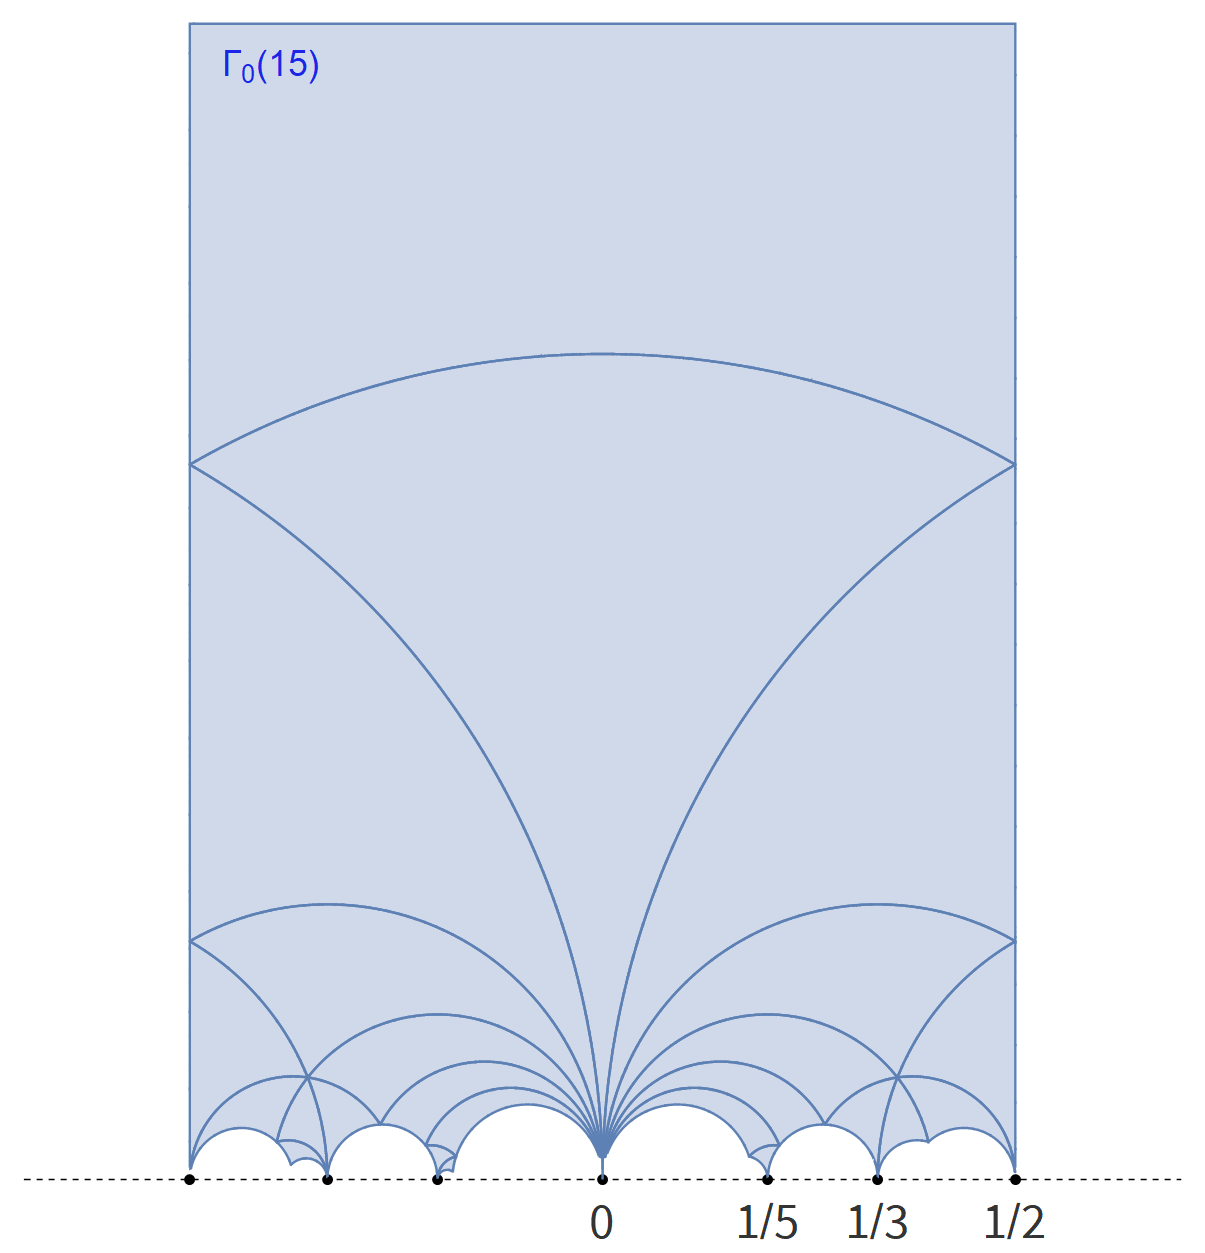
\includegraphics[scale=0.25]{figuras/domfundgamma015}
  \caption{El dominio fundamental del subgrupo de congruencia $\Gamma_0(15)$}
  \label{fig:domfunGamma15}
\end{figure}%%%%%%%%%%%%%%%%%%%%%%%%%%%%%%%%%%%%%%%%%%%%%%%%%%%%%%%%%%%%%%%%%%%%%%%%%%













\subsection{Formas Modulares y Operadores de Hecke}%%%%%%%%%%%%%%%%%%%%%%%%%%%%%%%%%%%%%%%%%%

Ahora nos enfocamos en funciones holomorfas $f:\HH\ra\CC$ que se transforman de cierta manera bajo
la acci\'on de un subgrupo de congruencia $\Gamma$. No podemos restringirnos solamente a tales
funciones que son invariantes bajo la acci\'on de $\Gamma$ (i.e. las funciones holomorfas definidas
sobre $\HH/\Gamma$) porque dejamos afuera la gran mayor\'ia de la teor\'ia de formas modulares.

En esta secci\'on iremos construyendo poco a poco los requerimientos que necesita tener $f$ para
poder llamarla una forma modular. Despu\'es estudiamos cierto operadores entre los espacios de
formas modulares que nos permite ``cambiar'' de subgrupo de congruencia; estos operadores son
ejemplos de operadores de Hecke. 

Pimero definimos dos conceptos fundamentales:

\begin{defin}
  El \emph{factor de automorf\'ia} se define como la funci\'on:
  \[
    j:\GL_2(\RR)\times\CC\lra\CC \qquad j(\gamma,z)=cz+d\quad
    \mathrm{donde}\; \gamma=\mat{a}{b}{c}{d}.
  \]
  Para cada $\gamma\in\GL_2^+(\RR)$ definimos el $[\gamma]_k-$\emph{operador de peso} $k$ sobre el
  espacio de funciones holomorfas $f:\HH\ra\CC$, como:
  \[
    \big(f[\gamma]_k\big)(z)=(\det\gamma)^{k/2}j(\gamma,z)^{-k}f(\gamma z).
  \]
\end{defin}

\begin{notas}
  La f\'ormula de $f[\gamma]_k$ es multiplicativa, es decir
  $[\gamma\gamma']_k=[\gamma]_k[\gamma']_k$ como operadores. Adem\'as, como $j$ restringido a
  $\GL_2(\RR)\times\HH$ no se anula, entonces $f$ y $f[\gamma]_k$ tienen los mismos ceros y polos.
\end{notas}

Ahora estudiamos funciones holomorfas $f:\HH\ra\CC$ que son invariantes bajo ciertas clases de
$[\gamma]_k-$operadores. En particular vamos a estudiar cuando $\gamma\in\Gamma$, un subgrupo
de congruencia.

\begin{defin}
  Sea $\Gamma\subseteq\SL_2(\ZZ)$ un subgrupo de congruencia y $f:\HH\ra\CC$ una funci\'on
  holomorfa. Decimos que $f$ es \emph{d\'ebilmente modular de peso k con respecto de} $\Gamma$
  si es $[\gamma]_k-$invariante para toda $\gamma\in\Gamma$, es decir:
  \[
    f[\gamma]_k=f \qquad\forall\gamma\in\Gamma.
  \]
  Para abreviar, a veces decimos que $f$ es d\'ebilmente $(\Gamma,k)-$modular.
\end{defin}
\begin{nota}
  Si $-1\in\Gamma$, por ejemplo en el caso $\Gamma=\Gamma_0(N)$, entonces ser $(\Gamma,k)-$modular
  implica la ecuaci\'on $f(z)=(f[-1]_k)(z)=(-1)^kf(z)$. Si $k$ es impar, la \'unica funci\'on que
  cumple esa ecuaci\'on es $0$. Por lo tanto, si $k$ es impar y $-1\in\Gamma$, la \'unica
  funci\'on d\'ebilmente $(\Gamma,k)-$modular es la funci\'on cero.
\end{nota}
Observa que si $\Gamma$ es un subgrupo de congruencia, i.e. $\Gamma(N)\subseteq\Gamma$, entonces
una funci\'on holomorfa $f:\HH\ra\CC$ d\'ebilmente modular de peso $k$ con respecto de $\Gamma$
es una funci\'on $N\ZZ-$peri\'odica, en efecto: la pertenencia de la matriz
\[
  \mat{1}{N}{0}{1}\in\Gamma(N)\subseteq\Gamma,
\]
que corresponde a la transformaci\'on $z\mapsto z+N$, implica que $f(z)=f(z+N)$. Por lo tanto
$f$ es $N\ZZ-$peri\'odica.

Nuestro siguiente prop\'osito es extender la noci\'on de holomorf\'ia de $f:\HH\ra\CC$ al punto
$z=\infty$ para poder hablar de funciones holomorfas sobre $X(\Gamma)$ inducidas por $f$'s que
sean d\'ebilmente modulares de peso $k$ con respecto de $\Gamma$. Primero tomamos el m\'inimo
entero positivo $h$ tal que:
\[
  \mat{1}{h}{0}{1}\in\Gamma
\]
y por lo anterior, $f$ es $h\ZZ$-peri\'odica. Esto quiere decir que $f$ deciende a $\HH/h\ZZ$,
el espacio cociente de la acci\'on $h\ZZ\act\HH$ de traslaciones $\{z\mapsto z+hk\}_{k\in\ZZ}$; por
el momento, denotamos a este espacio cociente por $\widetilde{\HH}$. Por lo tanto existe una
funci\'on $\tilde{f}:\widetilde{\HH}\ra\CC$ tal que $f=\tilde{f}\circ\pi$, donde
$\pi:\HH\epi\widetilde{\HH}$ es la proyecci\'on natural (v\'ease el diagrama conmutativo
\ref{cd:fcilindro}).

Por otro lado, la funci\'on exponencial:
\[
  q_h:\HH\lra D \qquad\text{definido por}\quad z\mapsto e^{2\pi i z/h},
\]
donde $D=\{0<\abs{z}<1\}$, es otra funci\'on $h\ZZ-$peri\'odica, i.e. tambi\'en se factoriza a
trav\'es de $\widetilde{\HH}$. Pero a diferencia de $\tilde{f}$, la funci\'on inducida
$\widetilde{q_h}:\widetilde{\HH}\ra D$ tiene un inverso holomorfo
\[
  \widetilde{q_h}^{-1}(z+h\ZZ)=\frac{h\log z}{2\pi i}
\]
que est\'a bien definido m\'odulo $h\ZZ$ porque $\log(z)=\log\abs{z}+i\arg(z)$ est\'a bien definido
m\'odulo $2\pi i\ZZ$.

Por lo tanto a $f$ le podemos asociar la funci\'on holomorfa $f_{\text{cil}}:D\ra\CC$ definido por
$f_{\text{cil}}=\tilde{f}\circ\widetilde{q_h}^{-1}$, aparece como la flecha punteada en el siguiente
diagrama:
\begin{equation}\label{cd:fcilindro}
  \begin{tikzcd}[row sep=25,column sep=30]
    \HH \arrow[dd,"q_h"'] \arrow[rrd, bend left=20, "f"] \arrow[dr, twoheadrightarrow] && \\
    &\widetilde{\HH} \arrow[ld, bend right=10,"\widetilde{q_h}"'] \arrow[r, "\tilde{f}"'] & \CC\\
    D \arrow[ru, bend right=10,near end, "\widetilde{q_h}^{-1}"']
    \arrow[rru, bend right=20, dashed,"f_{\text{cil}}"'] &&
  \end{tikzcd}
\end{equation}
La notaci\'on viene de ``cilindro'' pues $D$ es homeomorfo al cilindro.

La conmutatividad del diagrama implica que $f(z)=f_{\mathrm{cil}}(e^{2\pi i z/h})$ para toda.
$z\in\HH$. Como $\Im(z)\rai$ si y solamente si $e^{2\pi i z/h}\ra 0$, podemos interpretar que el
comportamiento de $f_{\text{cil}}$ cerca de 0 es an\'alogo al comportamiento de $f$ cerca de $\infty$.
Esto nos sugiere la siguiente definici\'on:

\begin{defin}
  Sea $f:\HH\ra\CC$ d\'ebilmente modular de peso $k$ con respecto de un subgrupo de congruencia
  $\Gamma$. Decimos que una funci\'on $f$ es \emph{holomorfa en} $\infty$ si la funci\'on holomorfa
  $f_{\mathrm{cil}}:D\ra\CC$ inducida admite una extensi\'on holomorfa a $D\cup\{0\}$ y decimos que
  se \emph{anula en} $\infty$ cuando la extensi\'on holomorfa si anula en 0. Si $f$ es holomorfa en
  $\infty$ la extensi\'on $\what{f_{\mathrm{cil}}}:D\cup{0}\ra\CC$ admite una serie de Taylor
  alrededor de $0$; sus coeficientes los denotamos por $a_n(f)$ y la serie la denotamos por:
  \[
    f_{\infty}(q)=\sum_{n=0}^{\infty}a_n(f)q^n\qquad\text{donde}\;\; q=e^{2\pi i z/h}\;\;(z\in\HH)
  \]
  donde $h$ es el m\'inimo entero positivo tal que $f(z)=f(z+h)$.
\end{defin}

\begin{notas}
  $f$ se anula en $\infty$ si y solamente si $a_0(f)=0$. Adem\'as, si $h=1$, como en el caso
  $\Gamma_0(N)$, entonces $f(z)=f(z+1)$ y la serie de Taylor $f_{\infty}(q)$ es simplemente la
  serie de Fourier de $f$. A veces decimos ``Fourier'' en lugar de ``Taylor'' si estamos en el
  caso de $\Gamma_0(N)$.
\end{notas}

La existencia de una extensi\'on holomorfa $\what{f_{\mathrm{cil}}}$ implica que $f_{\mathrm{cil}}$
es acotado cuando $q\ra0$. Gracias al comentario sobre el diagrama conmutativo (\ref{cd:fcilindro}),
esto es equivalente a que $\Im(f(z))$ es acotado cuando $\Im(z)\rai$. Por lo tanto tenemos una
condici\'on suficiente para que una funci\'on d\'ebilmente modular sea holomorfa en $\infty$:
\[
  f\;\;\text{es holomorfa en}\;\;\infty\quad\then\quad
  \big\{f(z_n)\big\}_{n\in\NN}\;\;\text{es acotado si}\;\;\lim_{n\rai}\Im(z_n)=\infty.
\]

Ahora que sabemos extender la noci\'on de holomorf\'ia a $\infty$, el siguiente paso es extenderlo
a las c\'uspides de un subgrupo de congruencia $\Gamma$. La idea es reducir el problema a considerar
holomorf\'ia en $\infty$.

Sea $f:\HH\ra\CC$ una func\'ion d\'ebilmente $(\Gamma,k)-$modular con $\Gamma$ de congruencia
y sea $z\in\QQ$ una c\'uspide de la acc\'ion $\Gamma\act\HH$. Sabemos que $z$ es de la forma
$z=a/c$ donde $a$ y $c$ son enteros primos relativos, entonces existen $b,d\in\ZZ$ tales que
$ad-bc=1$ y as\'i:
\[
  \mat{a}{b}{c}{d}\infty=\frac{a\infty+b}{c\infty+d}=\frac{a}{c}=z.
\]
En otras palabras, todas las c\'uspides de $\Gamma$ est\'an en la \'orbita
de $\infty$ bajo la acci\'on del grupo modular. Por lo tanto si $z\in\QQ$ es una c\'uspide de
$\Gamma\act\HH$, toma $\gamma\in\Gamma(1)$ tal que $z=\gamma\infty$. En este caso $\det\gamma=1$
y la restricci\'on $j(\gamma,*):\HH\ra\CC$ nunca se anula. Esto implica que $f[\gamma]_k$ es
holomorfa siempre y cuando $f$ lo sea.

Por otro lado, si $\tau\in\gamma^{-1}\Gamma\gamma$, entonces tiene la forma
$\tau=\gamma^{-1}\tau'\gamma$ y as\'i la igualdad:
\[
  \big(f[\gamma]_k\big)[\tau]_k=f[\gamma]_k[\gamma^{-1}\tau'\gamma]_k=f[\tau']_k[\gamma]_k
  \overset{*}{=}f[\gamma]_k,
\]
donde (*) se sigue de $\tau'\in\Gamma$ y $f$ siendo d\'ebilmente $(\Gamma,k)-$modular. Acabamos
de probar que $f[\gamma]_k$ es invariante bajo los $[\tau]_k-$operadores cuando
$\tau\in\gamma^{-1}\Gamma\gamma$, es decir $f[\gamma]_k$ es d\'ebilmente
$(\gamma^{-1}\Gamma\gamma,k)-$modular.\footnote{Podemos hablar de modularidad d\'ebil con respecto
  de $\gamma^{1}\Gamma\gamma$ porque \'este es un subgrupo de congruencia cuando $\Gamma$ lo es
  (c.f. \cite[\S1.4, lema 1.4.1]{BumpAFAR}).}
Por lo tanto tiene sentido hablar de holomorf\'ia en $\infty$ de la funci\'on $f[\gamma]_k$. Adem\'as,
simb\'olicamente tenemos que
\[
  ``\big(f[\gamma]_k\big)(\infty)=\det\gamma^{k/2}j(\gamma,\infty)^{-k}f(z)\text{''},
\]
lo cual sugiere expl\'icitamente c\'omo deber\'iamos de definir la holomorf\'ia en una c\'uspide
$z$ a partir de la holomorf\'ia de $f[\gamma]_k$ en $\infty$:

\begin{defin}
  Sea $f:\HH\ra\CC$ d\'ebilmente $(\Gamma,k)-$modular para alguna $\Gamma\subseteq\Gamma(1)$ de
  congruencia y $z\in\QQ$ una c\'uspide. Decimos que $f$ es \emph{holomorfa} en $z$ si $f[\gamma]_k$
  es holomorfa en $\infty$ donde $\gamma\in\Gamma(1)$ es tal que $z=\gamma\infty$.
\end{defin}

Observa que esta definici\'on no depende de la elecci\'on de $\gamma$. En efecto, la holomorf\'ia
de $f[\gamma]_k$ es independiente de la elecci\'on de $\gamma$ porque la acci\'on $z\mapsto\gamma z$
siempre es holomorfa.

Aunque no es tan inmediato, la condici\'on de anularse en $\infty$ tambi\'en es independiente de
$\gamma$. \emph{A priori}, las series de Fourier de $f[\gamma]_k$ y $f[\gamma']_k$ son distintas,
pero si $\gamma\infty=\gamma'\infty$, entonces las composiciones $f(\gamma z)$ y $f(\gamma'z)$ tiene
el mismo comportamiento cerca de $\infty$. Por lo tanto se anulan simultaneamente.

Ahora estamos en posici\'on para definir las formas modulares:

\begin{defin}
  Decimos que $f:\HH\ra\CC$ es una \emph{forma modular} de peso $k$ con respecto de un subgrupo de
  congruencia $\Gamma$ (o brevemente $(\Gamma,k)-$modular) si cumple las siguientes tres cosas:
  \begin{enumerate}[label=\emph{\roman*})]
  \item $f$ es holomorfo.
  \item $f[\gamma]_k=f$ para toda $\gamma\in\Gamma$, i.e. $f$ es d\'ebilmente $(\Gamma,k)-$modular.
  \item $f[\tau]_k$ es holomorfo en $\infty$ para toda $\tau\in\Gamma(1)$.
  \end{enumerate}
  Al conjunto de formas modulares de peso $k$ con respecto de $\Gamma$ se denota por $M_k(\Gamma)$.
  Si adem\'as cumple
  \begin{enumerate}[label=\emph{\roman*})]\setcounter{enumi}{3}
  \item $f[\tau]_k$ se anula en $\infty$ para toda $\tau\in\Gamma(1)$, i.e. $a_0(f[\tau]_k)=0$ para
    toda $\tau\in\Gamma(1)$.
  \end{enumerate}
  Decimos que $f$ es \emph{cuspidal}; el conjunto de formas modulares cuspidales se
  denota $S_k(\Gamma)$.
\end{defin}

En seguida enunciamos algunas propiedades b\'asicas de $M_k(\Gamma)$ y $S_k(\Gamma)$:

\begin{prop}\label{prop:prop_de_M}
 Sea $\Gamma\subseteq\SL_2(\ZZ)$ un subgrupo de congruencia. Entonces:
  \begin{enumerate}[label=\roman*)]
  \item $M_k(\Gamma)$ y $S_k(\Gamma)$ son $\CC-$espacios vectoriales de dimensi\'on finita.
  \item $\dim S_2(\Gamma)=g$ donde $g$ es el g\'enero de $X(\Gamma)$. En particular $S_2(\Gamma(1))=0$.
  \item\label{prop_de_M_3} $M(\Gamma):=\bigoplus_{k\geq0}M_k(\Gamma)$ es un anillo graduado y
    $S(\Gamma):=\bigoplus_{k\geq0}S_k(\Gamma)$ es un ideal.
  \item El espacio $S_k(\Gamma)$ admite un producto interior Hermitiano positivo-definido
    llamado el \emph{producto interior de Petersson}, definido por
    \[
      \gen{\textunderscore,\textunderscore}_{\Gamma}:S_k(\Gamma)\times S_k(\Gamma)\lra\CC\quad,\quad
      \gen{f,g}_{\Gamma}=\frac{1}{V_{\Gamma}}\int_{X(\Gamma)}f(z)\ol{g(z)}\im{z}^kd\mu(z)
    \]
    donde $\mu z=dxdy/y^2$ (donde $z=x+iy$) es la medida hiperb\'olica de $\HH$ y $V_{\Gamma}$ es
    el volumen hiperb\'olico%
    \footnote{Como $X(\Gamma)$ es una superficie de Riemann de primer tipo, su
      volumen es finito (c.f. \cite{FarkasKra})}\marginpar{buscar cita} de $X(\Gamma)$. i.e.
    $V_{\Gamma}=\int_{X(\Gamma)}d\mu$. A veces quitamos el ``$\Gamma$'' de la notaci\'on del producto
    interior cuando $\Gamma$ es claro del contexto.
  \end{enumerate}
\end{prop}

\begin{proof}
  El inciso $(i)$ es una aplicaci\'on cl\'asica del teorema de Riemann-Roch\footnote{Sea $X$ una
    curva completa, no singular sobre un campo algebraicamente cerrado de g\'enero $g$ (e.g. una
    superficie de Riemann compacta como una curva el\'iptica o $X(\Gamma)$). Sea $K$ el divisor
    can\'onico sobre $X$ y $D$ cualquier divisor. Entonces
    \[
      \ell(D)-\ell(K-D)=\deg D+1-g\quad,\quad\ell(D):=\dim H^0(X,\Ll(D))
    \]
    donde $H^0(X,\Ll(D))$ es el primer grupo de cohomolog\'ia de la gavilla invertible $\Ll(D)$
    asociada a $D$ bajo el isomofismo $\mathrm{Cl}(X)\cong\mathrm{Pic}(X)$ entre el grupo de
    divisores m\'odulo divisores principales y el grupo de Picard (c.f. el teorema 1.3 del
    cap\'itulo IV de \cite{HartshorneAG} para una prueba).}. El inciso $(ii)$ se sigue de que
  $f\mapsto fdz$ es un isomorfismo entre $S_2(\Gamma)$ y el espacio de 1-formas diferenciales
  sobre $X_0(N)$ (c.f. el corolario 2.17 de \cite{ShimuraITTATOAF}). La igualdad $\dim S_2(\Gamma)=g$
  se deduce (otra vez) de Riemann-Roch y el caso particular se sigue de que
  $X(\Gamma(1))=\HH^*/\Gamma(1)\approx\what{\CC}$, la esfera de Riemann. El
  $(iii)$ es trivial pues $M_k(\Gamma)\cdot M_{k'}(\Gamma)\subseteq M_{k+k'}(\Gamma)$. La prueba
  del inciso $(iv)$ es elemental pero un poco t\'ecnica, entonces referimos al lector a $\S 5.4$
  de \cite{DiamondShurmanAFCIMF}.
\end{proof}

Ahora estudiamos c\'omo transformar formas modulares en $M_k(\Gamma)$ a formas modulares en
$M_k(\Gamma')$ donde $\Gamma$ y $\Gamma'$ son dos subgrupos de congruencia. Primero necesitamos
lenguaje t\'ecnico de teor\'ia de grupos:

\begin{defin}
  Sean $\Gamma,\Gamma'\subseteq\SL_2(\ZZ)$ subgrupos de congruencia y sea $\alpha\in\GL_2^+(\QQ)$.
  Definimos la \emph{clase bilateral} de $\alpha$ con respecto de $\Gamma$ y $\Gamma'$ como el
  conjunto:
  \[
    \Gamma\alpha\Gamma'=\{\gamma\alpha\gamma'\in\GL_2^+(\QQ)\mid \gamma\in\Gamma,\,\gamma'\in\Gamma'\}.
  \]
\end{defin}

La multiplicaci\'on por la izquierda induce una acci\'on $\Gamma\act\Gamma\alpha\Gamma'$. Como
$\Gamma$ y $\Gamma'$ son de congruencia, entonces esta acci\'on particiona a la clase bilateral
en una cantidad finita de \'orbitas (c.f. lemas 5.1.1 y 5.1.2 de \cite{DiamondShurmanAFCIMF}),
m\'as precisamente:
\begin{equation}
  \label{eq:clasebilateralpart}
  \exists\beta_1,\ldots,\beta_n\in\Gamma\alpha\Gamma'\;\;\text{tal que}\;\;
  \Gamma\alpha\Gamma'=\bigsqcup_{i=1}^n\Gamma\beta_i,
\end{equation}
donde $\sqcup$ denota la uni\'on disjunta. Esta descomposici\'on de la clase bilateral nos permite
definir el siguiente operador:

\begin{defin}
  Sean $k\in\NN$, $\Gamma,\Gamma'\subseteq\SL_2(\ZZ)$ subgrupos de congruencia y sea
  $\Gamma\alpha\Gamma'$ una clase bilateral para alguna $\alpha\in\GL_2(\QQ)$. Definimos el
  $[\gag]_k-$operador como la funci\'on $[\gag]_k:M_k(\Gamma)\ra M_k(\Gamma')$ definida por
  \[
    f[\gag]_k=\sum_{i=1}^nf[\beta_i]_k,
  \]
  donde $\gag=\sqcup\Gamma\beta_i$ es una descomposici\'on como en (\ref{eq:clasebilateralpart}).
\end{defin}

\begin{nota}
  La definici\'on del $[\gag]_k-$operador es independiente de la descomposici\'on
  $\gag=\sqcup\Gamma\beta_i$. En efecto, si $\Gamma\beta=\Gamma\beta'$ para dos $\beta,\beta'\in\gag$
  donde $\beta=\gamma\alpha\gamma'$ y $\beta'=\delta\alpha\delta'$, tenemos que
  \[
    \alpha\gamma'=\gamma^{-1}\beta\in\Gamma\beta=\Gamma\beta'\quad\then\quad
    \alpha\gamma'=\sigma\beta'
    \quad\text{para alguna }\sigma\in\Gamma.
  \]
  De esta manera:
  \[
    f[\beta]_k=f[\gamma]_k[\alpha\gamma']_k= f[\gamma]_k[\sigma\beta']_k=f[\gamma\sigma]_k[\beta']_k
    \overset{*}{=} f[\beta']_k
  \]
  donde (*) se sigue de que $\gamma\sigma\in\Gamma$ y $f\in M_k(\Gamma)$. La igualdad anterior
  garantiza que $\sum f[\beta_i]_k$ es independiente de los representantes $\beta_1,\ldots,\beta_n$.

  Adem\'as, tenemos que el codominio de $[\gag]_k$ efectivamente es $M_k(\Gamma')$. Para verificar
  esto observa que la multiplicaci\'on por la derecha por $\gamma'\in\Gamma'$ en el espacio cociente
  $\Gamma\setminus\gag$ de la acci\'on izquierda $\Gamma\act\gag$ es una biyecci\'on
  bien definida:
  \[
    \Gamma\setminus\gag\lra\Gamma\setminus\gag \qquad\text{definido por}\quad
    \Gamma\delta\mapsto \Gamma\delta\gamma'.
  \]
  Por lo tanto sumar sobre los representantes $\{\beta_1,\ldots,\beta_n\}$
  de $\Gamma\setminus\gag$ es lo mismo que sumar sobre los representantes
  $\{\beta_1\gamma',\ldots,\beta_n\gamma'\}$. Por lo tanto si $f\in M_k(\Gamma)$, entonces para toda
  $\gamma'\in\Gamma'$ tenemos que:
  \[
    \big(f[\gag]_k\big)[\gamma']_k=\paren{\sum f [\beta_i]_k}[\gamma']_k=\sum f[\beta_i\gamma']_k=
    \sum f[\beta_i]_k=f[\gag]_k.
  \]
  Esto quiere decir que $f[\gag]_k$ es invariante bajo el $[\gamma']_k-$operador para toda
  $\gamma'\in\Gamma'$, es decir que $f[\gag]_k$ es d\'ebilmente $(\Gamma',k)-$modular. Lo que le
  falta a $f[\gag]_k$ para ser una forma modular es que sea holomorfo en $\infty$, pero esto se
  sigue del siguiente lema sencillo:

  \begin{lema}
    Sean $f_1,\ldots,f_m:\HH\ra\CC$ funciones donde cada $f_i$ es $h_i\ZZ-$peri\'odica y holomorfa en $\infty$.
    Entonces $f_1+\cdots+f_m$ es holomorfa en $\infty$.
  \end{lema}
  \begin{proof}
    Toma $h\in\ZZ^+$ como el m\'inimo com\'un m\'ultiplo de $h_1,\ldots,h_m$. Entonces
    $f:=f_1+\cdots+f_m$ es $h\ZZ-$peri\'odico. Por lo tanto $f_{\mathrm{cil}}$ existe y su
    extensi\'on holomorfa $\what{f_{\mathrm{cil}}}$ es la suma de las extensiones
    holomorfas $\what{f_{i,\mathrm{cil}}}$ de cada $f_{i,\mathrm{cil}}$ inducida por cada $f_i$.
    Como la suma de funciones holomorfas es holomorfa, $f_{\mathrm{cil}}$ admite una extensi\'on
    holomorfa al cero y por lo tanto $f_1+\cdots+f_m$ es holomorfa en $\infty$.
  \end{proof}

  Hemos probado que el codominio del $[\gag]_k-$operador es efectivamente $M_k(\Gamma')$.
\end{nota}

Enseguida estudiamos un caso importante de los $[\Gamma\alpha\Gamma']_k-$operadores. Primero sea
\begin{equation}\label{eq:alphap}
  \alpha_p=\mat{1}{0}{0}{p}\in\GL_2^+(\QQ),
\end{equation}
que corresponde a la transformaci\'on $z\mapsto z/p$. Entonces el $[\Gamma\alpha_p\Gamma']-$operador
es muy importante:

\begin{defin}
  Sea $p$ un n\'umero primo, $k\in\NN$ y $\Gamma\subseteq\SL_2(\ZZ)$ un subgrupo de congruencia.
  El $p-$\emph{\'esimo operador de Hecke de peso} $k$ \emph{con respecto de} $\Gamma$ es el operador
  $T_p:M_k(\Gamma)\ra M_k(\Gamma)$ definido por la clase lateral $\Gamma\alpha_p\Gamma$, i.e.
  $T_p=[\Gamma\alpha_p\Gamma]_k$ (v\'ease (\ref{eq:alphap}) para la definici\'on de $\alpha_p$).
\end{defin}

Resulta que si $p$ y $q$ son primos distintos, entonces sus respectivos operadores de Hecke
conmutan (v\'ease la proposici\'on \ref{prop:opdeHecke} m\'as adelante). Entonces si pudieramos
extender la definici\'on del $p-$\'esimo operador de Hecke para incluir potencias de primos
$p^{\beta}$ entonces podr\'iamos usar la factorizaci\'on \'unica de los enteros para extender la
definici\'on de operador de Hecke para que incluya a todo entero. Pero para esto necesitamos
introducir otro tipo de operador:

Recuerde que hay un epimorfismo $\Gamma_0(N)\epi(\ZZ/N\ZZ)^*$ con n\'ucleo $\Gamma_1(N)$
(c.f. la secci\'on \ref{sec:subgruposdecongruencia}). Entonces $\Gamma_1(N)$ es un subgrupo normal
de $\Gamma_0(N)$. As\'i, cuando $\alpha\in\Gamma_0(N)$, tenemos que
$\alpha^{-1}\Gamma_1(N)\alpha=\Gamma_1(N)$ y por lo tanto el cociente
$\Gamma_1(N)\setminus\Gamma_1(N)\alpha\Gamma_1(N)$ tiene solamente un elemento: $\Gamma_1(N)\alpha$.
De esta manera, si $f\in M_k(\Gamma_1(N))$, entonces:
\[
  f[\Gamma_1(N)\alpha\Gamma_1(N)]_k=f[\alpha]_k\qquad(\alpha\in\Gamma_0(N)).
\]
Esta f\'ormula induce una acci\'on de grupos $\Gamma_0(N)\act M_k(\Gamma_1(N))$ que, restringido
a $\Gamma_1(N)$ act\'ua trivialmente por definici\'on de $M_k(\Gamma_1(N))$. Por lo tanto la
acci\'on desciende al cociente $\Gamma_0(N)/\Gamma_1(N)\cong(\ZZ/N\ZZ)^*$. Esto quiere decir que
podemos definir la siguiente clase de operadores:

\begin{defin}
  Sea $d\in(\ZZ/N\ZZ)^*$ (o en general $d\in\ZZ$ con $(d,N)=1$). El operador \emph{diamante} se
  define como la funci\'on $\gen{d}:M_k(\Gamma_1(N))\ra M_k(\Gamma_1(N))$ definido por:
  \[
    \gen{d}f=f[\alpha]_k\quad\text{donde}\quad
    \alpha=\mat{a}{b}{c}{d'}\in\Gamma_0(N)\;\;\text{y}\;\; d\equiv d'\Mod{N}.
  \]
\end{defin}

Una propiedad importante que cumplen los operadores diamante es:

\begin{prop}\label{prop:chieigenespacios}
  Sea $G$ el grupo dual de Pontryagin del grupo finito $\ZZ/N\ZZ$, i.e.  $G=\Hom((\ZZ/N\ZZ)^*,\CC^*)$.
  Entonces $M_k(\Gamma_1(N))$ admite la siguiente descomposici\'on:
  \[
    M_k(\Gamma_1(N))=\bigoplus_{\chi\in G}M_k(\Gamma_1(N),\chi),
  \]
  donde definimos
  \[
    M_k(\Gamma_1(N),\chi)=
    \Big\{f\in M_k(\Gamma_1(N)) \,\Big|\, \gen{d}f=\chi(d)f\quad\forall d\in(\ZZ/N\ZZ)^*\Big\}.
  \]
\end{prop}
\begin{proof}
  Definimos una funci\'on $G\ra\End(M_k(\Gamma_1(N)))$ con $\chi\mapsto \pi_{\chi}$ donde
  \[
    \pi_{\chi}=\frac{1}{\phi(N)}\sum_{d\in(\ZZ/N\ZZ)^*}\chi(d)^{-1}\gen{d}
  \]
  como operadores. Para $\chi,\chi'\in G$ y $f\in M_k(\Gamma_1(N))$ tenemos que:
  \begin{align*}
    \pi_{\chi'}\pi_{\chi}(f)
    &=\pi_{\chi'}\paren{\frac{1}{\phi(N)}\sum_d\chi(d)^{-1}\gen{d}f}
      =\frac{1}{\phi(N)}\sum_d\chi(d)^{-1}\pi_{\chi'}\big(\gen{d}f\big)\\
    &=\frac{1}{\phi(N)}\sum_d\chi(d)^{-1}\paren{\frac{1}{\phi(N)}\sum_e\chi'(e)^{-1}\gen{e}\gen{d}f}\\
    &=\frac{1}{\phi(N)}\sum_d\chi(d)^{-1}\chi'(d)
      \paren{\frac{1}{\phi(N)}\sum_e\chi'(ed)^{-1}\gen{ed}f},
  \end{align*}
  donde $\gen{e}\gen{d}=\gen{ed}$ por la proposici\'on \ref{prop:opdeHecke} abajo.  
  Como $e\mapsto de$ es una permutaci\'on de $(\ZZ/N\ZZ)^*$, lo que est\'a en par\'entesis es
  simplemente $\pi_{\chi'}(f)$ que, por cierto, no depende de $d$. De las relaciones de
  ortogonalidad bien conocidas que cumplen los caracteres de grupos finitos\footnote{V\'ease, por ejemplo,
    el cap\'itulo 16, $\S3$ de \cite{IrelandRosenACITMNT} y en particular la proposici\'on 16.3.1.}
  obtenemos:
  \[
    \pi_{\chi'}\pi_{\chi}(f)=\pi_{\chi'}(f)\paren{\frac{1}{\phi(N)}\sum_d\chi(d)^{-1}\chi'(d)}=
    \begin{cases}
      \pi_{\chi'}(f) &\chi=\chi'\\
      0 &\chi\neq\chi'
    \end{cases}.
  \]
  Simb\'olicamente
  \begin{equation}
    \label{eq:proyeccionpichi}
    \pi_{\chi}^2=\pi_{\chi}\quad\text{y}\quad \pi_{\chi'}\pi_{\chi}=0 \quad (\chi\neq\chi').
  \end{equation}
  Ahora, si $f\in M_k(\Gamma_1(N))$ tenemos las siguientes dos igualdades:
  \begin{align*}
    \gen{d}\pi_{\chi}(f)=\frac{1}{\phi(N)}\sum_e\chi(e)^{-1}\gen{de}(f)
    &=\frac{\chi(d)}{\phi(N)}\paren{\sum_e\chi(de)^{-1}\gen{de}f}=\chi(d)\pi_{\chi}f,\\
    \paren{\sum_{\chi\in G}\pi_{\chi}}(f)=\sum_{\chi}\frac{1}{\phi(N)}\sum_d\chi(d)^{-1}\gen{d}f
    &=\sum_d\paren{\frac{1}{\phi(N)}\sum_{\chi}\chi(d)^{-1}}\gen{d}f\overset{*}{=}\gen{1}f=f,
  \end{align*}
  donde $(*)$ se sigue del hecho de que la suma dentro de los par\'entesis suma 0 cuando $d\neq1$.\footnote{Como
    $d\neq1$, $d$ determina un caracter no trivial del grupo finito $G$ y es conocido que la suma de todos los
    valores un caracter no trivial es 0. Este argumento est\'a en la prueba de la proposici\'on 16.3.1 de
    \cite{IrelandRosenACITMNT}.}
  Estas dos igualdades implican respectivamente que
  \begin{equation}
    \label{eq:proyeccionpichi2}
    \pi_{\chi}(M_k(\Gamma_1(N)))\subseteq M_k(\Gamma_1(N),\chi) \quad\text{y}\quad
    \sum_{\chi\in G}\pi_{\chi}=\Id.
  \end{equation}
  Por \'ultimo, si adem\'as $f\in M_k(\Gamma_1(N),\chi)$ entonces:
  \[
    \pi_{\chi}(f)=\frac{1}{\phi(N)}\sum_d\chi(d)^{-1}\gen{d}f=
    \frac{1}{\phi(N)}\sum_d\chi(d)^{-1}\chi(d)f=f\paren{\frac{1}{\phi(N)}\sum_d1}=f
  \]
  y por lo tanto
  \begin{equation}\label{eq:proyeccionpichi3}
    \pi_{\chi}|_{M_{k}(\Gamma_1(N),\chi)}=\Id.
  \end{equation}

  De \eqref{eq:proyeccionpichi}, \eqref{eq:proyeccionpichi2}  y \eqref{eq:proyeccionpichi3} se sigue
  que $M_k(\Gamma_1(N),\chi)$ es un sumando directo de $M_k(\Gamma_1(N))$. De la segunda parte de
  (\ref{eq:proyeccionpichi2}) se sigue que los subespacios $M_k(\Gamma_1(N),\chi)$ generan a
  $M_k(\Gamma_1(N))$ y de la segunda parte de (\ref{eq:proyeccionpichi}) se sigue que la
  intersecci\'on de esos subespacios es trivial. Por lo tanto $M_k(\Gamma_1(N))$ es la suma directa
  de sus subespacios $M_k(\Gamma_1(N),\chi)$ donde $\chi$ corre sobre $G$.
\end{proof}

Estos dos tipos de operadores cumplen muchas propiedades, entre ellas:

\begin{prop}\label{prop:opdeHecke} Sean $e,d\in(\ZZ/N\ZZ)^*$ y $p,q\in\ZZ$ primos. Entonces:
  \begin{enumerate}[label=\roman*)]
  \item $\gen{d}T_p=T_p\gen{d}$.
  \item $\gen{d}\gen{e}=\gen{de}=\gen{e}\gen{d}$
  \item $T_pT_q=T_qT_p$ cuando $p\neq q$.
  \item\label{prop:FourieropdeHecke} Si $f\in M_k(\Gamma_1(N))$ entonces la serie de
    Fourier de $T_pf$ es:
    \[
      (T_pf)_{\infty}(q)=
      \sum_{n=0}^{\infty}a_{pn}(f)q^n+p^{k-1}\sum_{n=0}^{\infty}a_n\big(\gen{p}f\big)q^{np}\quad
      (q=e^{2\pi i z}).
    \]
  \end{enumerate}
\end{prop}

\begin{proof}
  Esto es exactamente la proposici\'on 5.2.4 de \cite{DiamondShurmanAFCIMF}.
\end{proof}

De una manera similar a los caracteres de Dirichlet, podemos extender la definici\'on del operador
diamante $\gen{d}:M_k(\Gamma_1(N))\ra M_k(\Gamma_1(N))$ para $d$ cualquier entero. Adem\'as, para extender
la definici\'on de $T_p$, requerimos definir $T_{p^{\beta}}$ inductivamente usando los operadores
diamante $\gen{p}$.
\begin{defin}
  Sea $n\in\ZZ^+$, entonces definimos el operador diamante
  $\gen{n}:M_k(\Gamma_1(N))\ra M_k(\Gamma_1(N))$ como
  \[
    \gen{n}=
    \begin{cases}
      \gen{n} & (N,n)=1\\
      0 & (N,n)>1
    \end{cases}.
  \]
  Adem\'as, si $n=p_1^{\beta_1}\cdots p_m^{\beta_m}$ definimos $T_n:M_k(\Gamma)\ra M_k(\Gamma)$
  como el producto $T_n=T_{p_1^{\beta_1}}\cdots T_{p_m^{\beta_m}}$ donde cada $T_{p_i^{\beta_i}}$ se
  define inductivamente como:
  \[
    T_{p^{\beta}}=T_pT_{p^{\beta-1}}-p^{k-1}\gen{p}T_{p^{\beta-2}}.
  \]
\end{defin}

\begin{notas}
  El operador $\gen{n}$ es completamente multiplicativa, i.e. $\gen{nm}=\gen{n}\gen{m}$ para todas
  $n,m\in\ZZ$. Adem\'as es inmediato que $\gen{n}$ sigue conmutando con $T_m$ como en la proposici\'on
  \ref{prop:opdeHecke}.$i$:
  \begin{equation}
    \label{eq:Tnconmuta}
    T_m\gen{n}=\gen{n}T_m\qquad\forall n,m\in\ZZ^+.
  \end{equation}
  Por otro lado las $T_m$'s no siempre conmutan. Solamente tenemos
  \begin{equation}
    \label{eq:Tnconmutaprimo}
    T_mT_n=T_{nm}=T_nT_m\qquad\forall (n,m)=1
  \end{equation}
  por un argumento de inducci\'on sobre la definici\'on de $T_{p^{\beta}}$.
\end{notas}
\begin{nota}
  Con respecto del producto interior de Petersson, si $p\nmid N$, el operador adjunto de
  $\gen{p}$ es $\gen{p^{-1}}$ (donde $p^{-1}$ es el inverso de $p\mod N$) y el operador adjunto de $T_p$ es $\gen{p^{-1}}T_p$ (c.f. el teorema
  5.5.3 de \cite{DiamondShurmanAFCIMF}). Por lo tanto la proposici\'on \ref{prop:opdeHecke} nos
  garantiza que $\gen{p}$ y $T_p$ son operadores normales (i.e. conmutan con su operador adjunto)
  de la cual se sigue el siguiente resultado:
\end{nota}

\begin{prop}
  Sea $(n,N)=1$. Los operadores de Hecke $\gen{n},T_n:S_k(\Gamma_1(N))\ra S_k(\Gamma_1(N))$ son
  operadores normales con respecto del producto interior de Petersson.
\end{prop}
\begin{cor}\label{cor:basesimultanea}
  El espacio $S_k(\Gamma_1(N))$ tiene una base ortogonal de vectores propios simult\'aneos para
  los operadores de Hecke $\{\gen{n},T_n\mid (n,N)=1\}$.
\end{cor}
\begin{proof}
  El teorema espectral de \'algebra lineal para operadores normales.
\end{proof}

Los operadores de Hecke act\'uan sobre las series de Fourier de la siguiente manera:

\begin{prop}\label{prop:coefTnf}
  Sea $f\in M_k(\Gamma_1(N))$ con serie de Fourier $f_{\infty}(q)=\sum_{m\geq1}a_m(f)q^m$ donde
  $q=e^{2\pi i z}$. Entonces los coeficientes de Fourier de $T_nf$ est\'an dados por
  \[
    a_m(T_nf)=\sum_{d\mid(m,n)}d^{k-1}a_{nm/d^2}\big(\gen{d}f\big).
  \]
  En particular, si $(n,m)=1$, la f\'ormula anterior se reduce a:
  \[
    a_m(T_nf)=a_{nm}(f).
  \]
\end{prop}
\begin{proof}
  c.f. a la proposici\'on 5.3.1 de \cite{DiamondShurmanAFCIMF}.
\end{proof}


\subsection{Formas primitivas}\label{sec:formas_primitivas}%%%%%%%%%%%%%%%%%%%%%%%%%%%%%%%%%%%%%%%%%%%%%%%%%%%%%%%%%%%%%%%%%%%%%

En la secci\'on pasada vimos c\'omo cambiar de subgrupo de congruencia con los
$[\Gamma\alpha\Gamma']-$operadores. Ahora estudiamos un caso particular importante: cambiar de
nivel.

Sean $N$ y $M$ dos niveles con $M\mid N$. Entonces hay dos maneras de encajar $S_k(\Gamma_0(M))$
en $S_k(\Gamma_0(N))$. La m\'as sencilla es simplemente la inclusi\'on: si
\[
  \gamma=\mat{a}{b}{c}{d}\in\Gamma_0(N),
\]
entonces $N\mid c$ y por la transitividad de la divisibilidad tenemos que  $M\mid c$. Por lo tanto
$\gamma\in\Gamma_0(M)$. De esta manera $\Gamma_0(N)\subseteq\Gamma_0(M)$ y as\'i
\[
  M\mid N\quad\then\quad S_k(\Gamma_0(M))\subseteq S_k(\Gamma_0(N)).
\]

La otra manera de encajar $S_k(\Gamma_0(M))$ en $S_k(\Gamma_0(N))$ es ``multiplicando el nivel
por un divisor
de $N/M$''. M\'as precisamente, sea $d$ un divisor de $N/M$ y definimos
\[
  \beta_d=\mat{d}{0}{0}{1}\in\GL_2^+(\QQ).
\]
Observe que, si $f\in S_k(\Gamma_0(M))$, entonces $f[\beta_d]_k(z)=d^{k/2}f(dz)$. Afirmamos que
$f[\beta_d]_k\in S_k(\Gamma_0(Md))\subseteq S_k(\Gamma_0(N))$. De hecho se cumple algo m\'as general:

\begin{lema}\label{lema:subir_nivel_formas}
  Si $f\in S_k(\Gamma_0(M))$ y $g(z)=f(dz)$, entonces $g\in S_k(\Gamma_0(Md))$. 
\end{lema}
\begin{proof}
  Sea $\gamma\in\Gamma_0(Md)$. Observe que $g(z)=f(dz)=f(\beta_dz)$. Entonces
  calculamos:
  \[
    \big(g[\gamma]_k\big)(z)
    =j(\gamma,z)^{-k}g(\gamma z)
    =j(\beta_d\gamma,z)^{-k}f(\beta_d\gamma z)
    %=d^{-k/2}f[\beta_d]_k(\gamma z)
    %=d^{-k/2}j(\gamma,z)^k\big(f[\beta_d]_k[\gamma]_k\big)(z)
  \]
  donde hemos usado $j(\gamma,z)=j(\gamma\beta_d, z)$ porque multiplicar $\gamma$ por $\beta_d$ no
  altera el segundo rengl\'on de $\gamma$. Ahora, observe que:
  \[
    \underset{\beta_d}{\mat{d}{0}{0}{1}}\underset{\gamma}{\mat{a}{b}{c}{e}}
    =\underset{\gamma'}{\mat{a}{bd}{c/d}{e}}\underset{\beta_d}{\mat{d}{0}{0}{1}}
  \]
  donde $\gamma'\in\Gamma_0(M)$ poque $Md\mid c$. Entonces
  \[
    \big(g[\gamma]_k\big)(z)
    =j(\gamma'\beta_d,z)^{-k}f(\gamma'\beta_d z)
    =j(\gamma'z)^{-k}f(\gamma'\beta_d z)
    =f[\gamma']_k(\beta_dz)
    =f(dz)=g(z)
  \]
  porque $f\in S_k(\Gamma_0(M))$. Por lo tanto $g\in S_k(\Gamma_0(Md))$.
\end{proof}

En conclusi\'on, si $M\mid N$ y $d\mid N/M$, la funci\'on $S_k(\Gamma_0(M))\ra S_k(\Gamma_0(N))$
definida por $f\mapsto f[\beta_d]_k$ est\'a bien definida. Adem\'as, la funci\'on es inyeciva porque
si $f[\beta_d]_k=0$ claramente $f=0$; est\'a la segunda manera de encajar $S_k(\Gamma_0(M))$ en
$S_k(\Gamma_0(N))$.

%Si tenemos  formas $f_1,\ldots,f_n\in S_k(\Gamma_0(M))$ podemos obtener una forma en
%$S_k(\Gamma_0(N))$ combinando ambos m\'etodos anteriores: incluimos $f$ en
%$S_k(\Gamma_0(N))$, aplicamos $f\mapsto f[\beta_d]_k$ donde $d$ es un divisor de $N/M$ o hacemos una combinaci\'on de ambos
%m\'etodos. Las formas de $S_k(\Gamma_0(N))$ que vienen de formas de $S_k(\Gamma_0(M))$ bajo alguna
%de estas transformaciones, las llamaremos ``viejas''. Estaremos interesados en las formas que
%\emph{no} provienen de alguna forma de nivel m\'as bajo, es decir las formas ``nuevas''.

Sea $d$ es un divisor de $N$ definimos la funci\'on:
\[
  \iota_d:S_k(\Gamma_0(N/d))\times S_k(\Gamma_0(N/d))\lra S_k(\Gamma_0(N))
  \quad\text{definido por}\quad (f,g)\mapsto f+g[\beta_d]_k.
\]
Definimos:
\begin{defin}
  El subespacio de $S_k(\Gamma_0(N))$ generado por las im\'agenes de $\{\iota_d: d\mid N\}$ se
  llama el \emph{subespacio de formas viejas} y se denota por:
  \[
    S_k^{\mathrm{old}}(\Gamma_0(N))
    =\sum_{d\mid N}\iota_d\big(S_k(\Gamma_0(N/d))\times S_k(\Gamma_0(N/d))\big).
  \]
  El complemento ortogonal del subespacio de formas viejas (con respecto del producto interior de
  Petersson) se llama el \emph{subespacio de formas nuevas} y se denota por:
  \[
    \Snew=\big(\Sold\big)^{\perp}.
  \]
\end{defin}
%\begin{nota}
%  Para definir $S_k^{\mathrm{old}}(\Gamma_0(N))$ no es necesario sumar sobre todos los divisores
%  de $N$. Basta tomar solamente los divisores primos.
%\end{nota}

Intuitivamente el espacio de fomas viejas son todas las formas de $\Gamma_0(N)$ que provienen de un
$\Gamma_0(M)$ de nivel m\'as bajo mediante una combinaci\'on lineal de los dos m\'etodos anteriormente
mencionados.

Estos dos subespacios son invariantes bajo la acción de los operadores de Hecke:

\begin{prop}\label{prop:snew}
  Sea $\Hh=\{T_n,\gen{n}:\Sk\ra\Sk\mid n>0\}$ la familia de los operadores de Hecke, entonces:
  \begin{enumerate}[label=\roman*)]
  \item Los subespacios $\Snew$ y $\Sold$ son estables bajo todos los operadores de Hecke, i.e. $\Hh-$invariantes.
  \item En particular, $\Snew$ y $\Sold$ ambos tienen bases ortogonales formadas por vectores
    propios simult\'aneos de los operadores $\{T_n,\gen{n}\mid(n,N)=1\}$.
%  \item (Atkin-Lehner) Sea $f\in\Sk$ con serie de Fourier $f_{\infty}(q)=\sum_{n\geq1}a_n(f)q^n$,
%    entonces:
%    \[
%      a_n(f)=0,\;\;\forall(n,N)=1\quad\iff\quad
%      \forall p\mid N,\;\exists f_p\in S_k(\Gamma_0(N/p))
%      \;\;\;\mathrm{tales}\,\mathrm{que}\;\;\;
%      f(z)=\sum_{p\mid N}f_p(pz).
%    \]
%    En este caso tenemos que $f\in\Sold$. 
  \end{enumerate}
\end{prop}
\begin{proof}\cite[\S5.7]{DiamondShurmanAFCIMF}
%  Los primeros dos incisos vienen en . La direcci\'on
%  ``$\Longleftarrow$'' es relativamente sencillo de verificar a diferencia de la direcci\'on
%  ``$\then$'' que es mucho m\'as complicado. Atkin y Lehner publicaron la primera prueba de
%  $(iii)$ en 1970 \cite{AtkinLehnerHOOG}. En \cite[\S5.7]{DiamondShurmanAFCIMF} viene una prueba
%  detallada debida a David Carlton.
\end{proof}

\begin{defin}\label{def:formaprimitiva}
  Sea $f\in S_k(\Gamma_0(N))$ distinto de 0. Decimos que es una \emph{eigenforma} si es un vector
  propio simultaneo de todos los operadores de Hecke $\{T_n,\gen{n}\}_{n\geq1}$. Si adem\'as
  $f\in\Snew$ y est\'a \emph{normalizada}, i.e. $a_1(f)=1$, decimos que $f$ es una
  \emph{forma primitiva}.
\end{defin}

\begin{nota}
  Puede suceder que una forma $f\in S_k$ no sea vector propio simultáneo para todo operador de Hecke pero s\'i lo sea para todos los operadores salvo una cantidad finita, e.g. la familia  $\{T_n,\gen{n}\mid (n,N)=1\}$. En
  este caso decimos que $f$ es una \emph{eigenforma fuera de} $N$. Similarmente, si $f$ es adem\'as una
  forma nueva normalizada, decimos que es una \emph{forma primitiva fuera de} $N$. Como esta condición es más general, la usaremos más seguido.
\end{nota}

Los coeficientes de Fourier de una forma primitiva son sus valores propios con respecto de los operadores de Hecke $\{T_n\mid n>0\}$, en efecto:

\begin{prop}\label{thm:valores_propios_Fourier}
	Sea $f\in\Sk$ una eigenforma (fuera de $N$) con coeficientes de Fourier $\la_n:=a_n(f)$. Entonces existe un caracter $\chi:(\ZZ/N\ZZ)^*\ra\CC^*$ tal que $f\in S_k(\Gamma_0(N),\chi)$ (cf. proposición \ref{prop:chieigenespacios}), en particular $\gen{n}f=\chi(n)f$ para todo $(n,N)=1$. Si $\la_1=0$, entonces $T_nf=0$ y $f\in\Sold$, Si $\la_1\neq0$ entonces:
	\[
		T_nf=\frac{\la_n}{\la_1}f\quad\qquad\forall(n,N)=1.
	\]
	En particular si $f$ está normalizada, i.e. $\la_1=1$, los valores propios de $f$ bajo los operadores $T_n$ son precisamente sus coeficientes de Fourier.
\end{prop}
\begin{proof}
  Por hip\'otesis $f$ es vector propio simultaneo para los operadores $\{T_n,\gen{n}\mid(n,N)=1\}$,
  es decir existen $b_n,c_n\in\CC$ tales que
  \begin{equation}
    \label{eigennotacion}
    T_nf=b_nf\quad\text{y}\quad \gen{n}f=c_nf\qquad\text{donde}\;(n,N)=1.
  \end{equation}
  Por las propiedades del los operadores diamante, tenemos:
  \[
    c_{nm}f=\gen{nm}f=\gen{n}\gen{m}f=\gen{n}(c_mf)=c_mc_nf.
  \]
  Entonces $c_{nm}=c_nc_m$, lo cual quiere decir que la funci\'on $n\mapsto c_n$ es un caracter
  $\chi:(\ZZ/N\ZZ)^*\ra\CC^*$. En particular $\gen{n}f=c_nf=\chi(n)f$ y as\'i
  $f\in S_k(\Gamma_0(N),\chi)$.

  Solamente nos falta probar que $T_nf=(\la_n/\la_1)f$. Para esto calculamos $a_1(T_nf)$ de dos maneras distintas. Ya tenemos una fórmula general para calcular $a_1(T_nf)$ en la proposici\'on \ref{prop:coefTnf}. Por esta vía tenemos:
  \begin{equation}
    \label{eq:anf}
    a_1(T_nf)=a_n(f)=\la_n\qquad\forall n>0.
  \end{equation}
  Por el otro lado, $f$ es una eigenforma fuera de $N$, entonces por \eqref{eigennotacion} tenemos
  \begin{equation}
    \label{eq:anf2}
    \la_n=a_1(T_nf)=a_1(b_nf)=b_n a_1(f)=b_n\la_1.
  \end{equation}
 Aquí llegamos a dos casos: si $\la_1\neq0$, entonces tenemos
  \begin{equation}
    \label{eigenfourier}
    \frac{\la_n}{\la_1}=b_n \qquad \forall\; (n,N)=1.
  \end{equation}
	Pero si $\la_1=0$ entonces $\la_n=0$ para toda $(n,N)=1$. Por un resultado famoso debido a Atkin y Lehner publicado en en 1970, $f$ necesariamente es una forma vieja, i.e. $f\in\Sold$, \cite{AtkinLehnerHOOG}. En \cite[\S5.7]{DiamondShurmanAFCIMF} viene una prueba detallada debida a David Carlton.
\end{proof}


\begin{comment}%%%%%%%%%%%%%%%%%%%%%%%%%%%%%%%%%%%%%%%%%%%%%%%%%%%%%%%%%%%%%%%%%%%%%%%%%%%%%%%%%%%%%%%% ATKIN LEHNER,newFORM
Para probar esto primero necesitamos un lema que es consecuencia del teorema de Atkin-Lehner:

\begin{lema}\label{lema:sold}
  Si $f\in S_k(\Gamma_0(N))$ es una eigenforma fuera de $N$ y $a_1(f)=0$, entonces $f\in\Sold$.
\end{lema}
\begin{proof}
  Por hip\'otesis $f$ es vector propio simultaneo para los operadores $\{T_n,\gen{n}\mid(n,N)=1\}$,
  es decir existen $b_n,c_n\in\CC$ tales que
  \begin{equation}
    \label{eigennotacion}
    T_nf=b_nf\quad\text{y}\quad \gen{n}f=c_nf\qquad\text{donde}\;(n,N)=1.
  \end{equation}
  Por un lado tenemos:
  \[
    c_{nm}f=\gen{nm}f=\gen{n}\gen{m}f=\gen{n}(c_mf)=c_mc_nf,
  \]
  entonces $c_{nm}=c_nc_m$. Lo cual quiere decir que la funci\'on $n\mapsto c_n$ es un caracter
  $\chi:(\ZZ/N\ZZ)^*\ra\CC^*$. En particular $\gen{n}f=c_nf=\chi(n)f$ y as\'i
  $f\in S_k(\Gamma_0(N),\chi)$.

  Ahora, usamos la proposici\'on \ref{prop:coefTnf} para calcular $a_1(T_nf)$ para cualquier
  $n\in\ZZ^+$. Obtenemos
  \begin{equation}
    \label{eq:anf}
    a_1(T_nf)=a_n(f)\qquad\forall n\in\ZZ^+.
  \end{equation}
  Adem\'as, como $f$ es una eigenforma fuera de $N$, tenemos por otro lado que
  \begin{equation}
    \label{eq:anf2}
    a_1(T_nf)=a_1(b_nf)=b_n a_1(f).
  \end{equation}
  Si juntamos las dos f\'ormulas anteriores concluimos que
  \begin{equation}
    \label{eigenfourier}
    a_n(f)=b_n a_1(f) \qquad \forall\; (n,N)=1.
  \end{equation}

  Por hip\'otesis $a_1(f)=0$, entonces la f\'ormula \eqref{eigenfourier} implica que
  $a_n(f)=0$ para toda $(n,N)=1$. Por el teorema de Atkin-Lehner (proposici\'on \ref{prop:snew})
  tenemos que $f\in\Sold$.
\end{proof}

\begin{thm}\label{thm:valores_propios_Fourier}
  Sea $f\in\Snew$ una forma primitiva fuera de $N$, entonces los coeficientes de Fourier de $f$
  fuera de $N$ son
  sus valores propios con respecto a los operadores de Hecke fuera de $N$, es decir
  $T_nf=a_n(f)f$ para toda $(n,N)=1$.
\end{thm}
\begin{proof}
  Fijamos $m\geq1$ tal que $(m,N)=1$ y definimos $g_m=T_mf-a_m(f)f$; queremos probar que $g_m=0$.
  Como $\Snew$ es estable
  bajo $T_m$ (por la proposici\'on \ref{prop:snew}) entonces $T_mf\in\Snew$ y as\'i $g_m\in\Snew$.
  Por otro lado $g_m$ es una eigenforma fuera de $N$. Para ver esto,
  sea $n$ tal que $(n,N)=1$. Primero calculamos
  \[
    \gen{n}g_m=\gen{n}(T_mf-a_m(f)f)=T_m\gen{n}f-a_n(f)\gen{n}f=c_n(T_mf-a_m(f)f)=c_ng_m,
  \]
  donde $c_n$ es el valor propio de $f$ bajo $\gen{n}$ (c.f. la prueba lema \ref{lema:sold}). Por
  lo tanto $g_m$ es un vector propio  de $\gen{n}$ para toda $(n,N)=1$.

  Para ver que $g_m$ es un vector propio de $T_n$, tenemos que considerar primero el caso
  $n=p^{\alpha}$ para alg\'un primo $p$ y un exponente $\alpha\geq1$, y despu\'es usamos la
  definici\'on de $T_n$ para reducir la cuesti\'on al caso anterior.
  Primero sea $n=p^{\alpha}$ y hacemos inducci\'on. Para $\alpha=1$ tenemos
  \begin{align*}
    T_pg_m&=T_p(T_mf-a_m(f)f)=T_pT_mf-a_m(f)T_pf=T_p(b_mf)-a_m(f)b_pf=b_p(b_mf-a_m(f)f)\\ &=b_pg_m,
  \end{align*}
  donde hemos usado la notaci\'on de la ecuaci\'on \eqref{eigennotacion}.

  Ahora supongamos que $g_m$ es vector propio para los operadores
  $\{T_p,T_{p^2},\ldots,T_{p^{\alpha-1}}\}$ con valores propios $b_{p},b_{p^2},\ldots,b_{p^{\alpha-1}}$
  respectivamente. Con la f\'ormula recursiva de  $T_{p^{\alpha}}$ obtenemos:
  \begin{align*}
    T_{p^{\alpha}}g_m
    &=(T_pT_{p^{\alpha-1}}+p^{\alpha-1}\gen{p}T_{p^{\alpha-2}})g_m
      =T_pT_{p^{\alpha-1}}g_m+p^{\alpha-1}T_{p^{\alpha-2}}\gen{p}g_m\\
    &=T_p(b_{p^{\alpha-1}}g_m)+p^{\alpha-1}T_{p^{\alpha-2}}(c_pg_m)
      =\big(b_pb_{p^{\alpha-1}}+p^{\alpha-1}b_{p^{\alpha-2}}c_p\big)g_m.
  \end{align*}
  Hemos probado que $g_m$ es un vector propio para todo operador en
  $\{T_{p^{\alpha}}\mid \alpha\geq1,\, (p,N)=1\}$.

  Con esto podemos probar que $g_m$ es vector propio de $T_n$ para toda $(n,N)=1$. Primero sea
  $n=p_1^{\alpha_1}\cdots p_t^{\alpha_t}$ la factorizaci\'on \'unica de $n$. Como $g_m$ es vector
  propio de cada $T_{p_i^{\alpha_i}}$ por lo anterior, existen constantes $d_1,\ldots,d_t\in\CC$
  tales que $T_{p_i^{\alpha_i}}g_m=d_ig_m$. Con esto calculamos:
  \[
    T_ng_m=
    T_{p_1^{\alpha_1}}\cdots T_{p_t^{\alpha_t}}g_m=
    T_{p_1^{\alpha_1}}\cdots T_{p_{t-1}^{\alpha_{t-1}}}(d_tg_m)=\cdots=(d_1\cdots d_t)g_m
  \]
  y por lo tanto $g_m$ es un vector propio de $T_n$ para toda $(n,N)=1$, i.e. $g_m$ es una
  eigenforma fuera de $N$.

  Para poder aplicar el lema anterior, necesitamos calcular $a_1(g_m)$. Como  la funci\'on
  $f\mapsto a_1(f)$ es $\CC-$lineal, tenemos:
  \[
    a_1(g_m)
    =a_1(T_mf-a_m(f)f)
    =a_1(T_mf)-a_m(f)a_1(f)
    \overset{\eqref{eq:anf}}{=} a_m(f)\big(1-a_1(f)\big).
  \]
  Como $f$ es primitivo, est\'a normalizado, entonces la ecuaci\'on anterior se reduce a
  $a_1(g_m)=0$.
  Aplicamos el lema \ref{lema:sold} y deducimos que $g_m\in\Sold$. Ya ten\'iamos que
  $g_m\in\Snew=\Sold^{\perp}$, entonces $g_m=0$ y terminamos.
\end{proof}
\end{comment}%%%%%%%%%%%%%%%%%%%%%%%%%%%%%%%%%%%%%%%%%%%%%%%%%%%%%%%%%%%%%%%%%%%%%%%%%%%%%%%%%%%%%%%%%%%%%%%%%%%%%


Cerramos la secci\'on con una propiedad m\'as que cumplen las eigenformas:

\begin{prop}\label{prop:camponumerico}
  Sea $f\in S_k^{\mathrm{new}}(\Gamma_0(N),\chi)$ una forma primitiva. Entonces si denotamos
  $\la=\{a_n(f),\chi(n)\}_{n\geq1}$, la extensi\'on $\QQ(\la)$ de $\QQ$ es finita. Al campo
  $\QQ(\la)$ se denota por $K_f$ y se llama el \emph{campo num\'erico de} $f$.
\end{prop}
\begin{proof}\marginpar{buscar cita y poner prueba}%%%%%%%%%%%%%%%%%
  Para una prueba con geometr\'ia algebr\'aica, consulte
  \cite[proposici\'on 2.7.3 de \S2]{DeligneSerreFMDP1} o \cite[\S6.5]{DiamondShurmanAFCIMF}.
  En seguida escribimos una prueba elemental debida a Serre que aparece en \cite[\S2.5]{SerreMFOW1AGR}.

  Primero comentamos que $\QQ(a_n(f)\mid n\geq1)=\QQ(a_p(f)\mid p\,\text{es primo})$ porque cada $a_n(f)$ es un
  combinaci\'on algebr\'aica de las $a_p(f)$'s. Introducimos la
  siguiente notaci\'on: a cada forma primitiva $g\in S_k^{\mathrm{new}}(\Gamma_0(N),\chi)$ le
  asociamos su sistema de valores propios afuera de $N$ como el vector:
  \[
    \la(g)=\{a_p(g)\}_{p\nmid N}.
  \]
  Al conjunto de sistemas de valores propios lo denotamos por:
  \[
    \Lambda=\{\la(g)\mid g\in S_k(\Gamma_0(N),\chi)\;\text{es una forma primitiva}\}.
  \]
  Como $S_k(\Gamma_0(N),\chi)$ es de dimensi\'on finita, solamente puede haber una cantidad finita de
  sistemas de valores propios (c.f. corolario \ref{cor:basesimultanea}).
  Escribimos $\QQ(\chi)$ para denotar la extensi\'on de $\QQ$ por la imagen del caracter $\chi$ y
  denotamos $G=\Gal(\ol{\QQ}|\QQ(\chi))$. Este gupo de Galois act\'ua sobre los coeficientes de Fourier
  de las formas primitivas. M\'as precisamente, si $g\in S_k^{\mathrm{new}}(\Gamma_0(N),\chi)$ es una forma primitiva 
  con serie de Fourier $g(z)=\sum a_m(g)q^m$ y $\sigma\in G$, entonces definimos $g^{\sigma}$ con la
  serie de Fourier:\marginpar{explicar porque $a_n(f)\in\ol{\QQ}$}
  \[
    g^{\sigma}(z)=\sum_{m=1}^{\infty}a_m(g)^{\sigma}q^m,
  \]
  o en otras palabras, $a_m(g^{\sigma})=a_m(g)^{\sigma}$. Adem\'as, si escibimos $h:=\chi(n)g$, tenemos
  que:
  \[
    a_m(h^{\sigma})=a_m(h)^{\sigma}=(\chi(n)a_m(g))^{\sigma}=\chi^{\sigma}(n)a_m(g)^{\sigma}
                     =\chi(n)a_m(g^{\sigma})=a_m(\chi(n)g^{\sigma})\quad\;\big(\forall m\geq1\big)
  \]
  y por lo tanto $(\chi(n)g)^{\sigma}=\chi(n)g^{\sigma}$. Adem\'as citamos sin prueba que
  \[
    f\in S_k(\Gamma_0(N),\chi) \quad\then\quad f^{\sigma}\in S_k(\Gamma_0(N),\chi^{\sigma}).
  \]
  Una prueba para $k=2$ se encuentra en \cite[teorema 6.5.4]{DiamondShurmanAFCIMF} y el caso $k\geq2$ se
  encuentra en \cite[\S 3.5]{ShimuraITTATOAF}). Por \'ultimo para probar el caso $k=1$, se requiere de un truco
  t\'ecnico que aparece en la prueba que estamos siguiendo. Este resultado implica que:
  \begin{equation}\label{eq:diamsigma}
    \gen{n}g^{\sigma}=\chi^{\sigma}(n)g^{\sigma}=\chi(n)g^{\sigma}=(\chi(n)g)^{\sigma}=(\gen{n}g)^{\sigma}.
  \end{equation}
  

  Con esta notaci\'on y con la f\'ormula para calcular coeficientes de Fourier de $T_pg$
  (la proposici\'on \ref{prop:coefTnf}), tenemos que para $\sigma\in G$
  \begin{align*}
    a_m(T_pg)^{\sigma}&=\left( \sum_{d\mid (m,p)}d^{k-1}a_{pm/d^2}(\gen{d}g) \right)^{\sigma}
                      =\sum_d(d^{k-1})^{\sigma}\chi^{\sigma}(d)\big(a_{pm/d^2}(g)\big)^{\sigma}\\
                      &=\sum_dd^{k-1}\chi(d)\big(a_{pm/d^2}(g)\big)^{\sigma}
                        \qquad\big(\text{porque}\;\;\chi^{\sigma}=\chi\big)\\
                      &=\sum_dd^{k-1}\chi(d)a_{pm/d^2}(g^{\sigma})
                      =\sum_dd^{k-1}a_{pm/d^2}(\chi(d)g^{\sigma})\\
                      &\overset{\eqref{eq:diamsigma}}{=}\sum_dd^{k-1}a_{pm/d^2}(\gen{d}g^{\sigma})\\
                      &=a_m(T_pg^{\sigma}) \quad\forall m\geq1.\\
    \therefore\quad T_pg^{\sigma}&=(T_pg)^{\sigma}=\big(a_p(g)g\big)^{\sigma}=a_p(g)^{\sigma}g^{\sigma}.
  \end{align*}
  En otras palabras, $a_p(g)^{\sigma}$ es el valor propio de $g^{\sigma}$ bajo $T_p$. Por lo tanto tenemos
  una acci\'on de grupos $G\act \Lambda$ definido por $\la(g)\mapsto\la(g^{\sigma})$.

  Ahora fijamos $f\in S_k^{\mathrm{new}}(\Gamma_0(N),\chi)$. La \'orbita de $\la(f)\in\Lambda$, que
  es finita porque $\Lambda$ es finita, est\'a en biyecci\'on con $G/G_{\la(f)}$ donde
  $G_{\la(f)}=\{\sigma\in G\mid \la(f)=\la(f^{\sigma})\}$ es el estabilizador de $\la(f)$. Por lo tanto
  $G_{\la(f)}$ es de \'indice finito y as\'i $K$, el campo fijo de $G_{\la(f)}$ es una extensi\'on
  finita de $\QQ(\chi)$. Claramente cada entrada de $\la(f)$ es un elemento de $K$ pues si $\sigma\in G_{\la(f)}$
  tenemos que
  \[
    \{a_p(f)\}_{p\nmid N}=\la(f)=\la(f^{\sigma})=\{a_p(f)^{\sigma}\}_{p\nmid N}\quad\then\quad a_p(f)=a_p(f)^{\sigma}
    \quad\then\quad a_p(f)\in K\quad\forall p\nmid N.
  \]
  Como $K$ es una extensi\'on finita de $\QQ(\chi)$, tambi\'en es finita sobre $\QQ$  as\'i
  $K_f\subseteq K$ y $K_f$ es una extensi\'on finita de $\QQ$.
\end{proof}

\begin{nota}
  En la prueba con geometr\'ia algebraica de \cite{DeligneSerreFMDP1}, concluyen algo m\'as fuerte que $K_f$ sea una extensi\'on finita. Con sus m\'etodos deducen que adem\'as $a_n(f)\in\Oo_f$, el anillo de enteros de $K_f$. De esta manera es posible calcular congruencias m\'odulo ideales primos de $\Oo_f$; esto es un detalle importante para la prueba de la modularidad de $\rhot$ de la secci\'on \ref{sec:langlands_tunnell}.  En este trabajo solamente probamos que $K_f/\QQ$ es finito porque la prueba es elemental y m\'as concisa. Para una prueba m\'as detallada que la prueba de Deligne y Serre, v\'ease el teorema 6.5.1 de \cite{DiamondShurmanAFCIMF}.
\end{nota}

\subsection{Series de Eisenstein}\label{sec:eisenstein}%%%%%%%%%%%%%%%%%%%%%%%%%%%%%%%%%%%%%%%%%

Unos buenos ejemplos de formas modulares son las series de Eisenstein. Hay varios
estilos de series de Eisenstein, el m\'as sencillo se define como
\[
  E_{2k}(z):=\frac{1}{2}\sideset{}{'}\sum_{n,m\in\ZZ}\frac{1}{(mz+n)^{2k}} \qquad (k\geq 2),
\]
donde la notaci\'on $\Sigma'$ excluye el sumando $n=m=0$. Calculamos c\'omo se
transforman $E_{2k}$ bajo la acci\'on $\SL_2(\ZZ)\act\HH$.

Toda matriz
\[
  \gamma=
  \begin{pmatrix}
    a & b\\ c&d
  \end{pmatrix} \in \SL_2\ZZ
\]
induce una permutaci\'on
\[
  \ZZ\times\ZZ \lra \ZZ\times\ZZ \quad\text{definido por}\quad
  (m,n)\mapsto \gamma^t(m,n)=(am+cn,bm+dn)
\]
con inverso $(m,n)\mapsto (\gamma^t)^{-1}(m,n)$. En particular, como
$(0,0)\mapsto(0,0)$, la funci\'on anterior permuta los elementos de $\ZZ\times\ZZ-\{(0,0)\}$.
Por lo tanto:
\begin{align}
  E_{2k}\paren{\frac{az+b}{cz+d}}&=
  \frac{1}{2}\sideset{}{'}\sum_{n,m\in\ZZ}\frac{1}{(m\frac{az+b}{cz+d}+n)^{2k}}=
  \frac{1}{2}\sideset{}{'}\sum_{n,m\in\ZZ}\frac{(cz+d)^{2k}}{(maz+mb+ncz+d)^{2k}}\nonumber\\ & =
  \frac{(cz+d)^{2k}}{2}\sideset{}{'}\sum_{n,m\in\ZZ}\frac{1}{((ma+nc)z+(mb+nd))^{2k}}\nonumber\\ &=
  \frac{(cz+d)^{2k}}{2}\sideset{}{'}\sum_{n,m\in\ZZ}\frac{1}{(mz+n)^{2k}}\nonumber\\ & =
  (cz+d)^{2k}E_{2k}(z) \label{eq:eisenstein2k}.              
\end{align}

Para justificar la permutaci\'on de los sumandos, debemos probar que la serie definida por
$E_{2k}$ es absolutamente convergente. Para esto sean $\omega_1,\omega_2\in\CC^*$ tales que
$\tfrac{\omega_1}{\omega_2}=z$, entonces $L:=\ZZ\omega_1\oplus\ZZ\omega_2\subset\CC$ es una
ret\'icula, ie. $\{\omega_1,\omega_2\}$ es una $\RR$-base de $\CC$ (esto sucede porque
$\Im(\omega_1/\omega_2)=\Im(z)>0$ implica que $\omega_1$ y $\omega_2$ no son colineales).
De esta manera, si $\sigma\in\RR$:
\[
  \sideset{}{'}\sum_{n,m\in\ZZ}\frac{1}{\abs{mz+n}^{\sigma}}=
  \sideset{}{'}\sum_{n,m\in\ZZ}\frac{\omega_2^{\sigma}}{\abs{m\omega_1+n\omega_2}^{\sigma}}=
  \omega_2^{\sigma}\sideset{}{'}\sum_{\lambda\in L}\frac{1}{\abs{\lambda}^{\sigma}},
\]
otra vez, la notaci\'on $\Sigma'$ excluye el sumando $\lambda=0$ de la suma. Por lo tanto la
convergencia absoluta de la serie $E_{2k}$ se reduce a probar la convergencia del lado derecho.
Este fen\'omeno es bien conocido:

\begin{prop}\label{lema:conv_abs_sobre_reticula} %%%%%%%%%%%%%%%%%%%%%%%%%%%%%%%%%%%%%%% LEMA
  Sea $L=\ZZ\omega_1\oplus\ZZ\omega_2\subset\CC$ una ret\'icula, entonces:
  \[
    \sideset{}{'}\sum_{\lambda\in L}\frac{1}{\abs{\lambda}^{\sigma}}\;\;\text{converge}
    \quad\iff\quad\sigma>2
  \]
\end{prop}%%%%%%%%%%%%%%%%%%%%%%%%%%%%%%%%%%%%%%%%%%%%%%%%%%%%%%%%%%%%%%%%%%%%%%%%%%%%%%%%%%%%
\begin{comment}%%%%%%%%%%%%%%%%%%%%%%%%%%%%%%%%%%%%%%%%%%%%%%%%%%%%%%%%%%%%%%%%%%%%%%%%%%%%% COMMENT
\begin{proof}
Todos los elementos de $L-\{0\}$ est\'an sobre un paralelogramo con v\'ertices
$\{n\omega_1+n\omega_2,-n\omega_1+n\omega_2,-n\omega_1-n\omega_2,n\omega_1-n\omega_2\}$ para
alguna $n\geq 1$; a estos paralelogramos los denotamos por $P_n$. Observa que los puntos
de la ret\'icula sobre un lado de $P_n$ son $\{n\omega_1+k\omega_2\mid -n\leq k\leq n\}$.
En particular hay $2n+1$ puntos de la ret\'icula sobre un (y cualquier) lado del paralelogramo.
Por lo tanto hay $8n=4(2n+1)-4$ puntos en $L\cap P_n$ porque los cuatro v\'ertices se cuentan
dos veces. Adem\'as, la homotecia $z\mapsto nz$ lleva los v\'ertices $\pm m\omega_1\pm m\omega_2$ del
paralelogramo $P_m$ a los v\'ertices $\pm nm\omega_1\pm nm\omega_2$ del paralelogramo $P_{nm}$.
Es decir que $n P_m=P_{nm}$.

Ahora tomamos $r>0$ como la distancia m\'inima del $0\in\CC$ al primer paralelogramo $P_1$ y
$R>0$ como la distancia m\'axima del $0$ a $P_1$, ie. $R=\abs{\omega_1+\omega_2}$:

\begin{figure}[h]%%%%%%%%%%%%%%%%%%%%%%%%%%%%%%%%%%%%%%%%%%%%%%%%%%%%%%%%%%% FIGURA
  \centering
  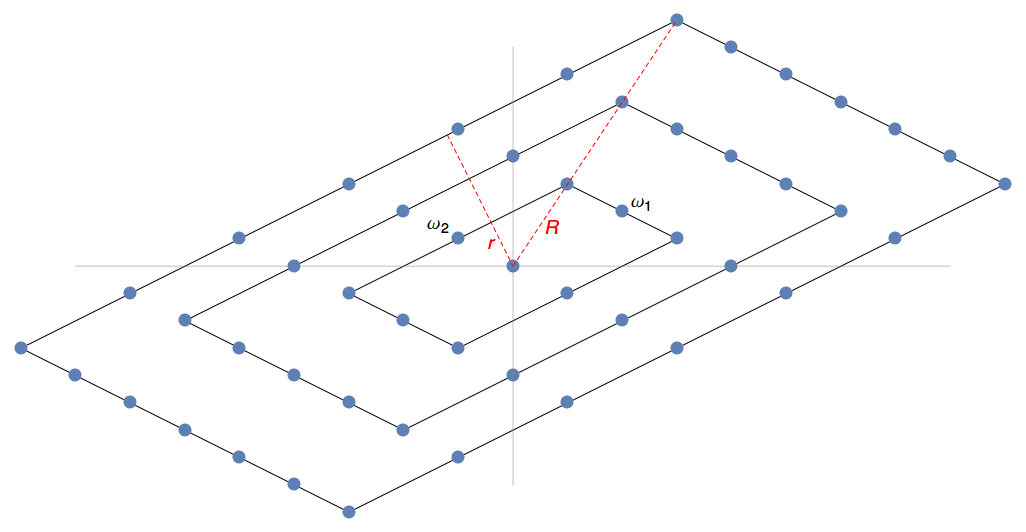
\includegraphics[scale=0.4]{reticula}
\end{figure}%%%%%%%%%%%%%%%%%%%%%%%%%%%%%%%%%%%%%%%%%%%%%%%%%%%%%%%%%%%%%%%%%%%%%%%%%%

\noindent De hecho podemos tomar $r$ como el radio de cualquier c\'irculo contenido en $P_1$
y $R$ como el radio de cualquier c\'irculo que contiene a $P_1$.

Entonces si $\lambda\in L\cap P_1$, tenemos que $r\leq\abs{\lambda}\leq R$. M\'as generalmente,
si $\lambda\in L\cap P_n=L\cap n P_1$ entonces $\lambda=n\lambda'$ con $\lambda'\in P_1$ y as\'i:
\[
  r\leq \abs{\lambda'}\leq R \quad\then\quad nr\leq\abs{\lambda}\leq nR
\]
Esta desigualdad implica que
\begin{equation}\label{eq:desigualdad_paralelogramo}
  \frac{1}{n^{\sigma}R^{\sigma}}\leq \frac{1}{\abs{\lambda}^{\sigma}}\leq
  \frac{1}{n^{\sigma}r^{\sigma}} \qquad(\lambda\in P_n\cap L).
\end{equation}

Ahora sumamos esta desigualdad sobre todos las $\lambda\in P_n\cap L$ y obtenemos:
\[
  \frac{8}{n^{\sigma-1}R^{\sigma}}\leq \sum_{\lambda\in P_n\cap L}\frac{1}{\abs{\lambda}^{\sigma}}\leq
  \frac{8}{n^{\sigma-1}r^{\sigma}}
\]
porque $\#(L\cap P_n)=8n$. Por \'ultimo, si ahora sumamos sobre todos los paralelogramos
hasta $P_N$ para alguna $N>0$, obtenemos:
\begin{equation}\label{eq:desigualdad_suma}
  \frac{8}{R^{\sigma}}\sum_{n=1}^N\frac{1}{n^{\sigma-1}}\leq
  \sum_{\underset{i\leq N}{\lambda\in P_i\cap L}}\frac{1}{\abs{\lambda}^{\sigma}}\leq
  \frac{8}{r^{\sigma}}\sum_{n=1}^N\frac{1}{n^{\sigma-1}}.
\end{equation} 

Ahora estamos en posici\'on de probar el lema: la cota superior de (\ref{eq:desigualdad_suma})
nos garantiza que si $\sigma>2$, la serie $\sum\abs{\lambda}^{-\sigma}$ converge porque el lado
derecho converge a $8r^{-\sigma}\zeta(\sigma-1)$ porque $\sigma-1>1$. Conversamente, si la serie
$\sum\abs{\lambda}^{-\sigma}$ converge, entonces el lado izquierdo converge a
$8R^{-\sigma}\zeta(\sigma-1)$ lo cual implica que $\sigma-1>1$ y terminamos.
\end{proof}
\end{comment} %%%%%%%%%%%%%%%%%%%%%%%%%%%%%%%%%%%%%%%%%%%%%%%%%%%%%%%%%%%%%%%%%%%%%%%% COMMENT

\begin{nota}
  Serre da dos pruebas en \cite[\S VII.2.2]{SerreACIA} y Shimura da otra prueba en
  \cite[\S III.8]{ShimuraMFBAB}.
\end{nota}

Por lo tanto, cuando $k\geq 2$, la f\'ormula \eqref{eq:eisenstein2k} es v\'alida y concluimos que
la serie de Eisenstein $E_{2k}$ es d\'ebilmente $(\Gamma(1),2k)-$modular. Para terminar de probar
que $E_{2k}$ es una forma modular, debemos probar que es holomorfa en $\infty$ (recuerde que
$\Gamma(1)$ solamente tiene una c\'uspide).

Es bien conocido (por ejemplo \cite[\S1.3, pg. 28]{BumpAFAR}) que $E_{2k}$ tiene la siguiente
expansi\'on en serie de Fourier:
\begin{equation}\label{eq:fourier_eisenstein2k}
  E_{2k}(z)=
  \zeta(2k)+\frac{(-1)^k(2\pi)^{2k}}{(2k-1)!}\sum_{n=1}^{\infty}\left(\sum_{d\mid n}d^{2k-1}\right)
  e^{2\pi inz}
\end{equation}
Esta f\'ormula claramente prueba que $E_{2k}(z)$ es holomorfa en $\infty$ porque no tiene
coeficientes negativos de Fourier. Concluimos que las f\'ormulas (\ref{eq:eisenstein2k}) y
(\ref{eq:fourier_eisenstein2k}) implican que $E_{2k}\in M_{2k}(\Gamma(1))$.

Si usamos los n\'umeros de Bernoulli y la identidad famosa
\[
  B_{2n}=(-1)^{n+1}\frac{2(2n)!}{(2\pi)^{2n}}\zeta(2n)\qquad (n>1)
\]
descubierta por Euler en 1735 \cite{EulerDSSR}, podemos reescribir la serie de Fourier como:
\[
  \frac{1}{\zeta(2k)}E_{2k}(z)=1-\frac{4k}{B_{2k}}\sum_{n=1}^{\infty}\sigma_{2k-1}(n)e^{2\pi inz}
\]
donde $\sigma_{2k-1}(n)$ es la notaci\'on cl\'asica para denotar $\sum_{d|n}d^{2k-1}$. Observa
que el primer coeficiente es 1; en este caso se dice que la serie $E'_{2k}(z):=\zeta(2k)^{-1}E_{2k}(z)$
est\'a normalizada.




\begin{comment}%%%%%%%%%%%%%%%%%%%%%%%%%%%%%%%%%%%%%%%%%%%%%%%%% #Bernoulli para deligne serre theorem
Lo interesante de la f\'ormula anterior es que podemos analizar mejor las propiedades de los
coeficientes de Fourier porque los n\'umeros de Bernoulli est\'an bien estudiados. En particular,
tenemos el teorema de von Staudt que dice:

\begin{thm}(von Staudt)%%%%%%%%%%%%%%%%%%%%%%%%%%%%%%%%%%%%%%%%%%%%%%%%%%%%%%%%%%%%%%%%% TEOREMA
  Si $l$ es un n\'umero primo y $l-1\mid m$, entonces $l B_m\in\ZZ_{(l)}$ y $$l B_m\equiv -1 \Mod{l}.$$
\end{thm}%%%%%%%%%%%%%%%%%%%%%%%%%%%%%%%%%%%%%%%%%%%%%%%%%%%%%%%%%%%%%%%%%%%%%%%%%%%%%%%%%%%%%%%

\begin{nota}
  Aqu\'i, $\ZZ_{(l)}$ es la localizaci\'on de $\ZZ$ con respecto del ideal primo $(l)\subset\ZZ$,
  es decir $\ZZ_{(l)}=\{\tfrac{a}{b}\in\QQ: p\not| \; b\}$. La prueba del teorema de von Staudt
  se basa en la relaci\'on entre los n\'umeros de Bernoulli y los valores de las sumas de potencias
  consecutivas, por ejemplo \cite[cap\'itulo 5, \S8, pg. 384]{ShafarevichNT}\footnote{Hay que tener
    cuidado con esta referencia porque en el enuciado del teorema escribe ``$l B_m\equiv 1$'' en lugar
    de ``$l B_m\equiv -1$''; esto parece ser un error de dedo porque en la prueba s\'i aparece el
    signo correcto.}.
\end{nota}

Con este teorema podemos probar una propiedad importante de las series de Eisenstein normalizadas:
su ``trivialidad m\'odulo $l$'' cuando $l-1$ divide al peso.

\begin{cor}\label{cor:eisenstien_trivial}%%%%%%%%%%%%%%%%%%%%%%%%%%%%%%%%%%%%%%%%%%%%%%%%%%%%
  Sea $l$ un n\'umero primo tal que $l-1\mid 2k$, y $E'_{2k}(z):=\sum a_ne^{2\pi inz}$ la serie
  de Fourier de la serie de Eisenstein normalizada de peso $2k$ (con $k>1$). Entonces todos los
  coeficientes son elementos de $\ZZ_{(l)}$ y
  \[
    a_m\equiv 0 \Mod{l} \qquad \forall m>0.
  \]
\end{cor}%%%%%%%%%%%%%%%%%%%%%%%%%%%%%%%%%%%%%%%%%%%%%%%%%%%%%%%%%%%%%%%%%%%%%%%%%%%%%%%%%%%%5
\begin{proof}
  Sea $B_{2k}=\tfrac{a}{b}\in\QQ$ con $(a,b)=1$. Por el teorema de von Staudt tenemos que
  $l B_{2k}\in\ZZ_{(l)}$ y que $l B_{2k}\equiv-1\Mod{l}$, es decir, existe $\frac{a'}{b'}\in\ZZ_{(l)}$
  tal que $l B_{2k}+1=l\tfrac{a'}{b'}$ o en particular $b'(la+b)=la'b$. Como $l\not|\;b'$, la
  igualdad anterior implica que $l|la+b$ y as\'i $l\mid b$. Observa que esto implica que $l\not|\;a$
  por la elecci\'on de $a$ y $b$. De esta manera tenemos:
  \[
    E'_{2k}(z)=
    1-\frac{4k}{B_{2k}}\sum_{n=1}^{\infty}\sigma_{2k-1}(n)e^{2\pi inz}=
    1-\sum_{n=1}^{\infty}\frac{4bk\sigma_{2k-1}(n)}{a}e^{2\pi inz}\in\ZZ_{(l)}[[e^{2\pi inz}]]
  \]
  y por \'ultimo, como $l\mid b$ y $l\not\,\mid a$ entonces $4bk\sigma_{2k-1}(n)/a\in l\ZZ_{(l)}$,
  que es otra manera de escribir la congruencia que quer\'iamos probar.
\end{proof}

Este corolario lo usaremos m\'as adelante en la prueba de un resultado debido a Deligne y Serre
(Secci\'on \ref{sec:DeligneSerre}).
\end{comment}%%%%%%%%%%%%%%%%%%%%%%%%%%%%%%%%%%%%%%%%%%%%%%%%%%%%%%%%%%%%%%%%%%%%%%%%%% COMMENT




En la prueba de STW semiestable, cuando se aplica el teorema de Langlands-Tunnell para probar la
modularidad de $\rhot$, aparece una serie de Eisenstein generalizada obtenida ``torciendo'' a $E_{2k}$
con un caracter de Dirichlet $\chi$. M\'as precisamente definimos
\[
  E_{k,\chi}(z):=\sideset{}{'}\sum_{n,m\in\ZZ}\frac{\chi(m)}{(mz+n)^k}
\]
donde $\chi$ es un caracter de Dirichlet.
El problema con esta serie es que en la demostraci\'on de la modularidad de $\rhot$, necesitamos
que el peso sea $k=1$ y la serie anterior no converge para este valor de $k$. Para poder evadir
este problema, introducimos un factor adicional que depende de un parametro complejo $s$:

\begin{defin}%%%%%%%%%%%%%%%%%%%%%%%%%%%%%%%%%%%%%%%%%%%%%%%%%%%%%%%%%%%%%%%%%%%%% DEFINICION
  Sea $k\in\ZZ$ y $\chi:(\ZZ/N\ZZ)^*\ra\CC^*$ un caracter de Dirichlet m\'odulo $N$,
  entonces la \emph{serie de Eisenstein de peso k, caracter $\chi$ y parametro} $s\in\CC$ se define como
  \[
    E_{k,\chi}(z,s):=\sum_{n,m\in\ZZ}\frac{\chi(m)}{(mz+n)^{k}\abs{mz+n}^{2s}}
  \]
  donde $z\in\HH$.
\end{defin}%%%%%%%%%%%%%%%%%%%%%%%%%%%%%%%%%%%%%%%%%%%%%%%%%%%%%%%%%%%%%%%%%%%%%%%%%%%%%%%%%%%

\begin{prop}
  La serie de Eisenstein $E_{k,\chi}$ satisface la ecuaci\'on de transfomaci\'on:
  \begin{equation}\label{eq:trans_eisenstein_gen}
  E_{k,\chi}(\gamma z,s) =(cz+d)^k\abs{cz+d}^{2s}\chi(d) E_{k,\chi}(z,s)
\qquad \Re(s)>1-\tfrac{k}{2}.
  \end{equation}
\end{prop}

\begin{proof}
Por proposici\'on \ref{lema:conv_abs_sobre_reticula} la serie $E_{k,\chi}(z,s)$ es absolutamente
convergente cuando $k+2\Re(s)>2$ o equivalentemente $\Re(s)>1-\frac{k}{2}$ (observa que el factor
$\chi(m)$ no afecta la convergencia absoluta porque $\abs{\chi(m)}=1$). Adem\'as la serie
es uniformemente convergente en cualquier conjunto compacto $K$ en el semiplano $\Re(s)>1-\frac{k}{2}$
porque para cualquier compacto en este semiplano, existe una $\eps>0$ tal que
$\Re(s)>1-\frac{k}{2}+\frac{\eps}{2}$ para toda $s\in K$. De esta manera $k+2\Re(s)>2+\eps$ y
tenemos que:
\[
  \sideset{}{'}\sum_{n,m\in\ZZ}\frac{1}{\abs{mz+n}^{k+2\Re(s)}}\leq
  \sideset{}{'}\sum_{n,m\in\ZZ}\frac{1}{\abs{mz+n}^{2+\eps}}<\infty \qquad(\forall s\in K).
\]
Por lo tanto la serie $E_{k,\chi}(z,s)$ es uniformemente convergente en $s$ sobre cualquier
compacto contenido en el semiplano $\Re(s)>1-\frac{k}{2}$. Por el teorema de Weierstrass, esto
implica que $E_{k,\chi}(z,s)$ define una funci\'on holomorfa en $s$ sobre el semiplano
$\Re(s)>1-\frac{k}{2}$.

Sea
\[
  \gamma=\begin{pmatrix}a & b\\ c&d\end{pmatrix} \in \Gamma_0(N)
\]
entonces:
\begin{align}
  E_{k,\chi}(\gamma z,s)&=
  \sideset{}{'}\sum_{n,m\in\ZZ}
  \frac{\chi(m)}{\paren{m\frac{az+b}{cz+d}+n}^k\abs{m\frac{az+b}{cz+d}+n}^{2s}}\nonumber\\ & =
  \sideset{}{'}\sum_{n,m\in\ZZ}%
  \frac{\chi(m)(cz+d)^k\abs{cz+d}^{2s}}{((ma+nc)z+(mb+nd))^k\abs{(ma+nc)z+(mb+nd)}^{2s}}\nonumber\\ & =
  (cz+d)^k\abs{cz+d}^{2s}\sideset{}{'}\sum_{n,n\in\ZZ}
  \frac{\chi(m)}{((ma+nc)z+(mb+nd))^k\abs{(ma+nc)z+(mb+nd)}^{2s}}.\label{eq:trans_eisenstein}
\end{align}
Ahora, como $\gamma\in\Gamma_0(N)\subset\SL_2\ZZ$ entonces $ad-bc=1$ lo cual implica que
$1\equiv ad-bc\equiv ad \Mod{N}$ y as\'i
\[
\chi(ma+cn)=\chi(ma)=\chi(m)\chi(a) \quad\then\quad
\chi(m)=\chi(ma+cn)\chi(d).
\]
Sustituimos esta f\'ormula para $\chi(m)$ en (\ref{eq:trans_eisenstein}) y recordamos que
$(m,n)\mapsto(ma+nc,mb+nd)$ permuta los elementos de $\ZZ\times\ZZ$ para concluir que:
\begin{align*}
  E_{k,\chi}(\gamma z,s)&=
  (cz+d)^k\abs{cz+d}^{2s}\chi(d)\sum_{n,n\in\ZZ}
  \frac{\chi(ma+nc)}{((ma+nc)z+(mb+nd))^k\abs{(ma+nc)z+(mb+nd)}^{2s}} \\ & =
  (cz+d)^k\abs{cz+d}^{2s}\chi(d)\sum_{n,m\in\ZZ}\frac{\chi(m)}{(mz+n)^{k}\abs{mz+n}^{2s}}
\end{align*}
Por lo tanto
\begin{equation*}
  E_{k,\chi}(\gamma z,s) =(cz+d)^k\abs{cz+d}^{2s}\chi(d) E_{k,\chi}(z,s),
\end{equation*}
y terminamos.
\end{proof}

Si hacemos $s=0$, entonces la f\'ormula anterior implicar\'ia que $E_{k,\chi}(z,0)$
se transforma adecuadamente para ser una forma modular en $M_k(\Gamma(1),\chi)$. El
problema es que la serie definida por $E_{k,\chi}(z,0)$ no converge si $k=1$ que es el
caso que nos interesa para la prueba de la modularidad de $\rhot$. Entonces lo que haremos
es continuar anal\'iticamente $E_{1,\chi}(z,s)$ a $s=0$ y que la continuaci\'on sea holomorfo
en $s=0$. De esta manera obtendremos una forma modular.

Este proceso es parte de un fen\'omeno m\'as general; nos referimos a \cite[\S7.2]{MiyakeMF} para
los detalles del caso general. En la aplicaci\'on del teorema de Langlands-Tunnel, se usa una serie
de Eisenstein particular de peso $k=1$ torcida por el s\'imbolo de Legendre m\'odulo 3 definido
por
\[
  \chi(m)=\leg{m}{3}=
  \begin{cases}
    1 & m\equiv 1 \Mod{3}\\
    -1 & m\equiv -1 \Mod{3}\\
    0 & m\equiv 0 \Mod{3}
  \end{cases}.
\]
Observemos que para cualquier caracter impar, i.e. $\chi(-1)=-1$, tenemos que
\begin{equation}\label{eq:chiimpar}
  \frac{\chi(-m)}{(-mz+n)\abs{-mz+n}^{2s}}=\frac{\chi(m)}{(mz-n)\abs{mz-n}^{2s}}.
\end{equation}
Por lo tanto obtenemos:

\begin{prop}
  Sea $k=1$ y $\chi$ un caracter de Dirichlet impar. Adem\'as definimos la funci\'on auxiliar
  \[
    \phi(z;s):=\frac{1}{z^{1+s}\bar{z}^s}\qquad(z\in\HH,\;\Re(s)>\tfrac{1}{2}).
  \]
  Con esta notaci\'on tenemos la siguiente identidad:
\begin{equation}\label{eq:E1chi}
  E_{1,\chi}(z,s)=
  2\sum_{m=1}^{\infty}\chi(m)m^{-1-2s}\sum_{r=0}^{m-1}
  \sum_{n'=-\infty}^{\infty}\phi\paren{z+\tfrac{r}{m}+n';s}\qquad(z\in\HH,\;\Re(s)>\tfrac{1}{2}).
\end{equation}
\end{prop}

\begin{proof}
Por la proposici\'on anterior, la serie $E_{1,\chi}(z,s)$ converge absolutamente cuando $\Re(s)>1/2$.
Como $\chi$ es impar, podemos usar \eqref{eq:chiimpar} para calcular:
\begin{align}
  E_{1,\chi}(z,s) & =\sideset{}{'}\sum_{n,m\in\ZZ}\frac{\chi(m)}{(mz+n)\abs{mz+n}^{2s}}\nonumber\\
                 & =\sum_{\underset{m\neq0}{m=-\infty}}^{\infty}\sum_{n=-\infty}^{\infty}
                   \frac{\chi(m)}{(mz+n)\abs{mz+n}^{2s}}\qquad(\text{porque}\;\chi(0)=0)\nonumber\\
                  & =\sum_{m=1}^{\infty}\sum_{n=-\infty}^{\infty}\frac{\chi(m)}{(mz+n)\abs{mz+n}^{2s}}+
                    \frac{\chi(-m)}{(-mz+n)\abs{-mz+n}^{2s}}\nonumber\\
                  & =\sum_{m=1}^{\infty}\chi(m)\sum_{n=-\infty}^{\infty}\frac{1}{(mz+n)\abs{mz+n}^{2s}}+
                    \frac{1}{(mz-n)\abs{mz-n}^{2s}}\nonumber\\
  \therefore E_{1,\chi}(z,s)& = 2\sum_{m=1}^{\infty}\chi(m)\sum_{n=-\infty}^{\infty}
                    \frac{1}{(mz+n)\abs{mz+n}^{2s}} \qquad (\Re(s)>\tfrac{1}{2}).\label{eq:primer_E1chi}
\end{align}
Podemos reescribir la serie $\sum(mz+n)^{-1}\abs{mz+n}^{-2s}$ en otra serie que nos permitir\'a expresar
$E_{1,\chi}(z,s)$ como una serie de Fourier. Primero observemos que:
\begin{align*}
  (mz+n)^{-1}\abs{mz+n}^{-2s}&=(mz+n)^{-1}(mz+n)^{-s}(\overline{mz+n})^{-s}
                             =(mz+n)^{-1-s}(m\bar{z}+n)^{-s}\\
                            &=m^{-1-2s}\paren{z+\tfrac{n}{m}}^{-1-s}\paren{\bar{z}+\tfrac{n}{m}}^{-s}.
\end{align*}
Ahora fijamos un $m$ y dividimos $\ZZ$ en las $m$ clases laterales $0+m\ZZ,1+m\ZZ,\ldots,(m-1)+m\ZZ$.
De esta manera, si $n\in r+m\ZZ$, entonces $n=n'm+r$ para alguna $n'\in\ZZ$ y as\'i:
\[
  (mz+n)^{-1}\abs{mz+n}^{-2s}=
  m^{-1-2s}\paren{z+\tfrac{r}{m}+n'}^{-1-s}\paren{\bar{z}+\tfrac{r}{m}+n'}^{-s}.
\]
Por lo tanto:
\begin{equation}\label{eq:intermediateE}
\sum_{n=-\infty}^{\infty}\frac{1}{(mz+n)\abs{mz+n}^{2s}} =
\sum_{r=0}^{m-1}\sum_{n'\in\ZZ}
\frac{m^{-1-2s}}{\paren{z+\tfrac{r}{m}+n'}^{1+s}\paren{\bar{z}+\tfrac{r}{m}+n'}^s}.
\end{equation}


podemos reescribir la ecuaci\'on \eqref{eq:intermediateE} como
\[
  \sum_{n=-\infty}^{\infty}\frac{1}{(mz+n)\abs{mz+n}^{2s}}=
  m^{-1-2s}\sum_{r=0}^{m-1}\sum_{n'=-\infty}^{\infty}\phi\paren{z+\tfrac{r}{m}+n';s}
\]
para que la ecuaci\'on \eqref{eq:primer_E1chi}, se reduzca a:
\begin{equation*}
  E_{1,\chi}(z,s)=
  2\sum_{m=1}^{\infty}\chi(m)m^{-1-2s}\sum_{r=0}^{m-1}
  \sum_{n'=-\infty}^{\infty}\phi\paren{z+\tfrac{r}{m}+n';s}\qquad(z\in\HH,\;\Re(s)>\tfrac{1}{2}).
\end{equation*}
\end{proof}

Introducimos m\'as notaci\'on: escribimos
\begin{equation}\label{eq:S}
  S(z;s):=\sum_{n=-\infty}^{\infty}\phi(z+n;s),\qquad z\in\HH,\;\Re(s)>\tfrac{1}{2}.
\end{equation}
Esta notaci\'on nos resume la ecuaci\'on \eqref{eq:E1chi} a:
\begin{equation}
  \label{eq:EviaS}
  E_{1,\chi}(z,s)=2\sum_{m=1}^{\infty}\chi(m)m^{-1-2s}\sum_{r=1}^{m-1}S\big(z+\tfrac{r}{m};s\big),
  \qquad z\in\HH,\;\Re(s)>\tfrac{1}{2}.
\end{equation}

En lo que sigue, vamos a desarrollar la serie de Fourier de $S$ como funci\'on de $x=\Re(z)$.
Para esto usamos las siguientes notaciones: para $z=x+iy\in\HH$,
\[
  \phi_{y,s}(x):=\phi(x+iy;s)\qquad,\qquad S_{y,s}(x):=S(x+iy;s).
\]
Fijamos $y>0$ y $s\in\CC$ tal que $\Re(s)>\tfrac{1}{2}$ junto con una constante $\tfrac{1}{2}<\delta<\Re(s)$.
Observe que
\begin{align}
  \abs{\phi(x+iy;s)}
  &=\abs{x+iy}^{-\Re(s)-1}\abs{x-iy}^{-\Re(s)}=|x+iy|^{-2\Re(s)-1},\label{eq:approxdephi}\\
    \therefore\quad|\phi_{y,s}(x)|
  &=O(|x|^{-2\delta-1}).\nonumber
\end{align}

\begin{lema}
  La serie
  \[
    S_{y,s}(x)=\sum_{n=-\infty}^{\infty}\phi_{y,s}(x+n)
  \]
converge absolutamente y uniformemente sobre $0\leq x\leq1$. En particular
$S_{y,s}(x)$ es una funci\'on continua sobre el intervalo $[0,1]$ y $1-$peri\'odico.
\end{lema}

\begin{proof}
Sea $0\leq x\leq1$. En este caso, \eqref{eq:approxdephi} implica que
\[
  |\phi_{y,s}(x+n)|=|x+n+iy|^{-2\Re(s)-1}\leq |n-1+iy|^{-2\Re(s)-1}
  =O(n^{-2\delta-1})\qquad (0\leq x\leq 1)
\]
y as\'i la serie $\sum\phi_{y,s}(x+n)$ converge absolutamente  uniformemente sobre el intervalo
$[0,1]$. Por lo tanto $S_{y,s}(x)$ es continua sobre el mismo intervalo. Por otro lado, es claro que
\[
  S_{y,s}(x+1)
  =\sum_{n\in\ZZ}\phi_{y,s}(x+n+1)
  =\sum_{n\in\ZZ}\phi_{y,s}(x+n)
  =S_{y,s}(x),
\]
y terminamos.
\end{proof}


Como consecuencia del lema anterior  $S_{y,s}$ tiene una serie de Fourier
$\sum a_m e^{2\pi imx}$ cuyos coeficientes son:
\begin{align*}
  a_m
  &=\int_0^1 S_{y,s}(x)e^{-2\pi imx}dx
    =\int_0^1\sum_{n\in\ZZ}\phi_{y,s}(x+n)e^{-2\pi imx}dx\\
  &=\sum_{n\in\ZZ}\int_0^1\phi_{y,s}(x+n)e^{-2\pi imx}dx
    =\sum_{n\in\ZZ}\int_n^{n+1}\phi_{y,s}(x)e^{-2\pi im(x-n)}dx\\
  &=\int_{-\infty}^{\infty}\phi_{y,s}(x)e^{-2\pi imx}dx\\
  \therefore\quad a_m
  &=\hat{\phi}_{y,s}(m),
\end{align*}
donde $\hat{\phi}_{y,s}$ denota su transformada de Fourier que,
por \eqref{eq:approxdephi}, existe cuando $\Re(s)>\tfrac{1}{2}$.

Para probar que $S_{y,s}$ es igual a su serie de Fourier, i.e.
\begin{equation}
  \label{eq:seriefourierS}
  S_{y,s}(x)=\sum_{n=-\infty}^{\infty}\hat{\phi}_{y,s}(n)e^{2\pi inx},
\end{equation}
solamente nos falta probar\footnote{Esto es un resultado est\'andar del
  an\'alsis de Fourier. V\'ease, por ejemplo, el corolario 2.3 de \cite{SteinFA}
para una prueba expl\'icita.} que la serie de Fourier converge absolutamente,
es decir:
\begin{equation}
  \label{eq:convabsphihat}
  \sum_{n=-\infty}^{\infty}|\hat{\phi}_{y,s}(n)|<\infty
  \qquad (y>0,\;\Re(s)>\tfrac{1}{2}).
\end{equation}
Para este fin tenemos la siguiente proposici\'on t\'ecnica que probamos en el ap\'endice
y que viene, de manera m\'as general, en \cite[\S7.2]{MiyakeMF}.

\begin{prop}\label{prop:de_phihat}
  Sean $y>0$ y $n\in\ZZ$ fijos y denota $\varphi_{y,n}(s):=\hat{\phi}_{y,s}(n)$. Entonces:
  \begin{enumerate}[label=\roman*)]
  \item $\varphi_{y,n}(s)$ es holomorfa en el semiplano $\HH'=\{z\in\CC\mid\Re(z)>0\}$.
  \item $\varphi_{y,n}(s)$ admite una extensi\'on holomorfa a todo $\CC$ definida por
    \begin{equation}\label{eq:formulaphihat}
      \varphi_{y,n}(s)=\hat{\phi}_{y,s}(n)=
      \begin{cases}
        \dfrac{i\pi^sn^{s-1}e^{-2\pi ny}}{2\Gamma(s)y^{s+1}}\st(4\pi ny;s,s+1) &n>0\\
        2\pi i(2y)^{-2s}\Gamma(2s)\Gamma(s)^{-1}\Gamma(s+1)^{-1} &n=0\\
        \dfrac{2i\pi^{s+1}|n|^se^{-2\pi|n|y}}{y^s\Gamma(s+1)}\st(4\pi|n|y;s+1,s) &n<0
      \end{cases}.
    \end{equation}
    donde
    \[
      \st(z;\alpha,\beta):=\frac{z^{\beta}}{\Gamma(\beta)}\int_0^{\infty}e^{-zw}(w+1)^{\alpha-1}w^{\beta-1}dw
      \qquad(\Re(z),\Re(\beta)>0,\alpha\in\CC)
    \]
    admite  una extensi\'on holomorfa a todo $\HH'\times\CC\times\CC$.
  \item\label{prop:inciso3} En particular:
    \[
      \varphi_{y,n}(0)=\hat{\phi}_{y,0}(n)=
      \begin{cases}
        0 & n>0\\
        2\pi i e^{2\pi ny} &n\leq0
      \end{cases}.
    \]
  \item\label{prop:inciso4} Para todo subconjunto compacto $Q\subset\CC$ existen constantes $A,B>0$
    tales que
    \[
      |\varphi_{y,n}(s)|=|\hat{\phi}_{y,s}(n)|\leq
      \begin{cases}
        A y^{-\Re(s)-1}n^{\Re(s)-1}(1+(4\pi ny)^{-B})e^{-2\pi ny} & n>0\\
        A y^{-\Re(s)}|n|^{\Re(s)}(1+(4\pi |n|y)^{-B})e^{-2\pi|n|y} & n<0
      \end{cases}.
    \]
  \end{enumerate}
\end{prop}

Con esta proposici\'on podemos probar la convergencia absoluta de la serie
de Fourier de $S_{y,s}$, i.e.
\[
  \sum_{n=-\infty}^{\infty}|\hat{\phi}_{y,s}(n)|<\infty,\qquad y>0,\; \Re(s)>\tfrac{1}{2},
\]
Para probar esto introducimos la siguiente notaci\'on:
\[
  S_{\pm}(z;s):=\sum_{\underset{n\neq0}{n=-\infty}}^{\infty}\hat{\phi}_{y,s}(n)e^{2\pi inx},
\]
y separamos esta serie en las dos series
\[
  S_+(z;s):=\sum_{n=1}^{\infty}\hat{\phi}_{y,s}(n)e^{2\pi inx}\quad\text{y}\quad
  S_-(z;s):=\sum_{n=1}^{\infty}\hat{\phi}_{y,s}(-n)e^{-2\pi inx}.
\]


\begin{cor}\label{thm:S_holomorfo_gen}%%%%%%%%%%%%%%%%%%%%%%%%%%%%%%%%%%%%%%%%%%%%%%%%%%%% TEOREMA
  $S(z;s)$ admite una continuaci\'on holomorfa a $\HH\times\{\Re(s)>-\tfrac{1}{2}\}$
  definida por la f\'ormula:
  \begin{equation}\label{eq:exp_fourier_S}
    S(z;s)
    =\sum_{\underset{n\neq0}{n=-\infty}}^{\infty}\hat{\phi}_{y,s}(n)e^{2\pi inx}
    =\hat{\phi}_{y,s}(0)+S_{\pm}(z;s),
    \qquad z=x+iy\in\HH,\; \Re(s)>-\tfrac{1}{2},
  \end{equation}
  donde $S_{\pm}$ es holomorfa sobre $\HH\times\CC$ y $\hat{\phi}_{y,s}(0)$ es
  meromorfa sobre $\HH\times\CC$ con polos en $s=-\tfrac{1}{2},-\tfrac{3}{2},-\tfrac{5}{2},\ldots$.
  Adem\'as, para todo compacto $Q\subset\HH\times\{\Re(s)>-\tfrac{1}{2}\}$,
  existen constantes $\eps,A,B,M>0$ tales que
  \[
    |S(z;s)|\leq A\sum_{n=1}^{\infty}n^M(1+(4\pi\eps n)^{-B})e^{-2\pi\eps n}
    \qquad\forall(z,s)\in Q.
  \]
%  En particular para $s=0$ tenemos:
%  \[
%    S(z;0)=\frac{2\pi i}{1-e^{-2\pi i z}}.
%  \]
\end{cor}%%%%%%%%%%%%%%%%%%%%%%%%%%%%%%%%%%%%%%%%%%%%%%%%%%%%%%%%%%%%%%%%%%%%%%%%%%%%%%%%%%%%
\begin{proof}
  Ya hab\'iamos mencionado en \eqref{eq:convabsphihat} que la f\'ormula \eqref{eq:exp_fourier_S}
  se siguir\'ia de 
  Con esta notaci\'on tenemos:
  \[
    S(z;s)=\hat{\phi}_{y,s}(0)+S_{\pm}(z;s)=\hat{\phi}_{y,s}(0)+S_+(z;s)+S_-(z;s).
  \]
  Probaremos que las series $S_+$ y $S_-$ convergen  absolutamente y uniformemente sobre
  cualquier subconjunto compacto de $\HH\times\CC$. Aqu\'i estamos usando t\'acitamente la
  proposici\'on anterior que define $\hat{\phi}_{y,s}$ para todo valor de $s\in\CC$.
  Todo esto implicar\'ia que la serie de Fourier $\sum\hat{\phi}_{y,s}(n)e^{2\pi inx}$ de
  $S_{y,s}$ converge absolutamente (y uniformemente); precisamente lo que necesitamos.
  Adem\'as implicar\'ia que $S_{\pm}(z;s)$ es holomorfa sobre $\HH\times\CC$. Procedemos
  a probar la convergencia absoluta y uniforme de $S_+$ y $S_-$ sobre compactos de
  $\HH\times\CC$.
  
  Sea $Q\subset\HH\times\CC$ un subconjunto compacto y $(z,s)\in Q$ donde $z=x+iy$.
  De una vez elegimos $\delta>0$ tal que $\delta<y$ para toda $(x+iy,s)\in Q$.
  Gracias a la aproximaci\'on de la proposici\'on \ref{prop:de_phihat} inciso
  \ref{prop:inciso4} existen constantes $A,B>0$ tales que:
  \begin{align*}
    |\hat{\phi}_{y,s}(n)|
    &\leq A y^{-\Re(s)-1}n^{\Re(s)-1}(1+(4\pi ny)^{-B})e^{-2\pi ny}\\
    &\leq A y^{-\Re(s)-1}n^{\Re(s)-1}(1+(4\pi n\delta)^{-B})e^{-2\pi n\delta},
      \quad\forall(z,s)\in Q\; n>0.
  \end{align*}
  Adem\'as $\Re(s)$ est\'a acotada superiormente por ejemplo $\Re(s)<M+1$, entonces
  $n^{\Re(s)-1}\leq n^M$ para toda $n\geq1$ y as\'i
  \begin{equation}\label{eq:phihataprox1}
    |\hat{\phi}_{y,s}(n)|\leq A y^{-\Re(s)-1}n^M(1+(4\pi n\delta)^{-B})e^{-2\pi n\delta},
    \quad\forall(z,s)\in Q\; n>0.
  \end{equation}
  Similarmente si $n<0$ y $(z,s)\in Q$ tenemos que
  \begin{equation}\label{eq:phihataprox2}
    |\hat{\phi}_{y,s}(n)|\leq A y^{-\Re(s)}|n|^{M+1}(1+(4\pi|n|\delta)^{-B})e^{-2\pi|n|\delta},
    \quad\forall(z,s)\in Q\; n<0.
  \end{equation}
  Entonces:
  \begin{align*}
    |S_+(z;s)|
    &=\abs{\sum_{n=1}^{\infty}\hat{\phi}_{y,s}(n)e^{2\pi i n x}}
    \leq\sum_{n=1}^{\infty}|\hat{\phi}_{y,s}(n)e^{2\pi i n x}|\\
    &\leq A y^{-\Re(s)-1}\sum_{n=1}^{\infty}n^M(1+(4\pi n\delta)^{-B})e^{-2\pi n\delta}
      \quad\forall (z,s)\in Q.
  \end{align*}
  Adem\'as, como $y^{-\Re(s)-1}$ es una funci\'on continua sobre $Q$,
  est\'a acotado por una constante que podemos tomar como $L/A>0$ para alguna $L>0$.
  Por lo tanto: para toda $(z,s)\in Q$ existen constantes $\delta,B,L,M>0$ tales que:
  \begin{equation}\label{eq:phi1cota}
    |S_+(z;s)|\leq L\sum_{n=1}^{\infty}n^M(1+(4\pi n\delta)^{-B})e^{-2\pi n\delta}<\infty.
  \end{equation}
  As\'i $S_+(z;s)$ converge absolutamente y uniformemente sobre $Q$ para todo
  compacto $Q\subset\HH\times\CC$. Similarmente para toda $(z,s)\in Q$,
  \[
    |S_-(z;s)|\leq L\sum_{n=1}^{\infty}n^{M+1}(1+(4\pi n\delta)^{-B})e^{-2\pi n\delta}<\infty,
  \]
  y por lo tanto la serie $S_-(z;s)$ converge absolutamente y uniformemente sobre
  cualquier subconjunto compacto de $\HH\times\CC$.
  Concluimos que $S_+$ y $S_-$ son funciones holomorfas sobre $\HH\times\CC$ y
  de esta manera, $S_{\pm}=S_++S_-$ tambi\'en es holomorfa sobre $\HH\times\CC$.
  Adem\'as, si cambiamos $M$ por $M+1$ en \eqref{eq:phi1cota} obtenemos
  \begin{equation}
    \label{eq:approxPhi}
    |S_{\pm}(z;s)|\leq 2A\sum_{n=1}^{\infty}n^{M+1}(1+(4\pi\eps n)^{-B})e^{-2\pi\eps n}.
  \end{equation}

  En particular, si $Q\subset\HH\times\{\Re(s)>-\tfrac{1}{2}\}$, el t\'ermino
  \[
    \hat{\phi}_{y,s}(0)=\frac{2\pi i(2y)^{-2s}\Gamma(2s)}{\Gamma(s)\Gamma(s+1)}
  \]
  es una funci\'on continua de $s$ pues $\Gamma(2s)/\Gamma(s)$ es continuo para $2s>-1$.
  Entonces $|\hat{\phi}_{y,s}(0)|$ es acotado por una constante $C>0$ sobre $Q$. Esta cota la
  absorbe la constante $A$ de \eqref{eq:approxPhi} y con esto deducimos la
  aproximaci\'on que necesit\'abamos demostrar.

  Por lo tanto podemos concluir que $S_{y,s}$ es igual a su serie de Fourier:
  \begin{equation}\label{eq:S_prel}
    S(z;s)=\hat{\phi}_{y,s}(0)+
    \sum_{\underset{n\neq0}{n=-\infty}}^{\infty}\hat{\phi}_{y,s}(n)e^{2\pi inx}=
    \underset{*}{\underbrace{\frac{2\pi i(2y)^{-2s}\Gamma(2s)}{\Gamma(s)\Gamma(s+1)}}}+S_{\pm}(z;s).
  \end{equation}
  Esto quiere decir que $S(z;s)$ es suma de la funci\'on holomorfa $S_{\pm}$ con el
  cociente (*) que es una funci\'on meromorfa con polos en
  $s=-\tfrac{1}{2},-\tfrac{3}{2},-\tfrac{5}{2}\ldots$, i.e. los polos de $\Gamma(2s)$
  que no son los polos de $\Gamma(s)$ ni de $\Gamma(s+1)$. Observe que como $2y$ es un
  real, no necesitamos definir una rama del logaritmo para que $(2y)^{-2s}$ sea holomorfa.
  Con todo esto, concluimos que el lado derecho de \eqref{eq:exp_fourier_S} es una funci\'on
  meromorfa que define una extensi\'on de $S(z;s)$ a $\HH\times\CC$.

  Por \'ultimo usamos el inciso \ref{prop:inciso3} de la proposici\'on
  \ref{prop:de_phihat} para calcular $S_{\pm}(z;0)$. Claramente tenemos
  que $S_+(z;0)=0$ y as\'i
  \[
    S_{\pm}(z;0)=
    S_-(z;0)=
    \sum_{n=1}^{\infty}\hat{\phi}_{y,0}(-n)e^{-2\pi inx}=
    2\pi i\sum_{n=1}^{\infty}e^{-2\pi in(x+iy)}=2\pi i\sum_{n=1}^{\infty}e^{-2\pi i nz}.
  \]
  Por lo tanto sustituimos $s=0$ en \eqref{eq:S_prel} para obtener
  \[
    S(z;0)=
    2\pi i\frac{(2y)^{-2\cdot0}\Gamma(2\cdot0)}{\Gamma(0)\Gamma(0+1)}+S_{\pm}(z;0)=
    2\pi i\sum_{n=0}^{\infty}e^{-2\pi i nz}=\frac{2\pi i}{1-e^{-2\pi i z}}.
  \]
\end{proof}






\begin{prop}%%%%%%%%%%%%%%%%%%%%%%%%%%%%%%%%%%%%%%%%%%%%%%%%%%%%%%%%%%%%%%%%%%% COROLARIO
  La serie de Eisenstein $E_{1,\chi}(z;s)$ admite una continuaci\'on anal\'itica a $s=0$ y
  por lo tanto $E_{1,\chi}(z;0)$ es una forma $(\Gamma(1),1)-$modular.
\end{prop}%%%%%%%%%%%%%%%%%%%%%%%%%%%%%%%%%%%%%%%%%%%%%%%%%%%%%%%%%%%%%%%%%%%%%%%%%%%%%%%%%

\begin{proof}
  Fijamos $m\geq1$ y usamos la f\'ormula de $S$ para calcular
  \[
    \sum_{r=0}^{m-1}S\paren{z+\tfrac{r}{m};s}
    =\sum_{r=0}^{m-1}\sum_{n=-\infty}^{\infty}\hat{\phi}_{y,s}(n)e^{2\pi in(x+r/m)}
    =\sum_{n=-\infty}^{\infty}\hat{\phi}_{y,s}(n)e^{2\pi inx}\sum_{r=0}^{m-1}e^{2\pi inxr/m}.
  \]
  Ahora,
  \[
    \sum_{r=0}^{m-1}(e^{2\pi in/m})^r=
    \begin{cases}
      m & m\mid n\\
      0 & m\nmid n
    \end{cases},
  \]
  donde el caso $m\nmid n$ se verifica porque estamos sumando varias veces todas
  las raices $m'-$\'esimas de la unidad que da cero, donde $m'=m/(n,m)$. Entonces tenemos que
  \[
    \sum_{r=0}^{m-1}S\paren{z+\tfrac{r}{m};s}=m\sum_{n\in m\ZZ}\hat{\phi}_{y,s}(n)e^{2\pi inx}.
  \]
  Sustituimos la expresi\'on anterior en la f\'ormula \eqref{eq:EviaS} de
  $E_{1,\chi}(z,s)$:
  \begin{align}
    E_{1,\chi}(z,s)
    &=2\sum_{m=1}^{\infty}\chi(m)m^{-1-2s}\sum_{r=0}^{m-1}S\paren{z+\tfrac{r}{m};s}\nonumber\\
    &=2\sum_{m=1}^{\infty}\sum_{n\in m\ZZ}\chi(m)m^{-2s}\hat{\phi}_{y,s}(n)e^{2\pi inx}\nonumber\\
    &=2\sum_{n\in\ZZ}\Big(\sum_{\underset{m>0}{m\mid n}}\chi(m)m^{-2s}\Big)\hat{\phi}_{y,s}(n)e^{2\pi inx}
      \qquad z\in\HH,\;\Re(s)>\tfrac{1}{2}.\label{eq:serieFourierEpre}
  \end{align}

  Ahora, si $s\in\CC$ es tal que $\Re(s)>-\tfrac{1}{2}$ o equivalentemente $-2\Re(s)<1$,
  tenemos que $m^{-2\Re(s)}<m$ y as\'i
  \[
    \Big| \sum_{\underset{m>0}{m\mid n}}\chi(m)m^{-2s} \Big|\leq
    \sum_{m\mid n}|\chi(m)|m^{-2\Re(s)}<\sum_{m\mid n}m<n^2,\qquad\Re(s)>-\tfrac{1}{2}.
  \]
  De esto es claro que la serie del lado derecho de \eqref{eq:serieFourierEpre}
  converge absolutamente y uniformemente sobre cualquier subconjunto compacto $Q$
  de $\HH\times\{\Re(s)>-\tfrac{1}{2}\}$. En efecto las f\'ormulas \eqref{eq:phihataprox1}
  y \eqref{eq:phihataprox2} nos dan una cota uniforme de $\hat{\phi}_{y,s}(n)$ para $(z,s)\in Q$
  que decae exponencialmente en $n$ (observe que $y^{\Re(s)}$ es una funci\'on continua
  de $y$ y as\'i est\'a acotado para toda $(z,s)\in Q$).

  Por lo tanto el lado derecho de \eqref{eq:serieFourierEpre}, como funci\'on de
  $(z,s)$ define una funci\'on  holomorfa sobre $\HH\times\{\Re(s)>-\tfrac{1}{2}\}$.
  Como la igualdad \eqref{eq:serieFourierEpre} es sobre el abierto
  $\HH\times\{\Re(s)>\tfrac{1}{2}\}$, esta igualdad define una extensi\'on holomorfa
  de $E_{1,\chi}(z,s)$ a $\HH\times\{\Re(s)>-\tfrac{1}{2}\}$.

  En la f\'ormula \eqref{eq:serieFourierEpre} ponemos $s=0$ y usamos la proposici\'on
  \ref{prop:de_phihat} inciso \ref{prop:inciso3} para calcular:
  \begin{align*}
    E_{1,\chi}(z,0)
    &=2\sum_{n\in\ZZ}\Big(\sum_{\underset{m>0}{m\mid n}}\chi(m)\Big)\hat{\phi}_{y,0}(n)e^{2\pi inx}\\
    &=4\pi i\sum_{n=-\infty}^{0}\Big(\sum_{\underset{m>0}{m\mid n}}\chi(m)\Big)e^{2\pi ny}e^{2\pi inx}\\
    &= 4\pi i\sum_{n=0}^{\infty}\Big(\sum_{\underset{m>0}{m\mid n}}\chi(m)\Big)e^{-2\pi inz}.
  \end{align*}
  


  

\end{proof}

\end{document}
